% This template was partially made with assistance from Microsoft Co-pilot

% ------------------------------------------------------------------
% CAPSTONE SOFTWARE REQUIREMENTS SPECIFICATION (SRS)

% 
% This template is inspired by IEEE 29148 but simplified for use in 
% a senior software engineering capstone project. 
% 
% The goal is not to maximize document length. 
% The goal is to produce a clear, testable, and traceable set of 
% requirements that can guide design, implementation, and testing. 
% 
% Recommended workflow: 
% Stakeholder Requirements 
% -> 
% Use Cases 
% -> 
% Functional Requirements 
% -> 
% Acceptance Tests (will be in your VnV plan)
% -> 
% Traceability Matrix (will excluded traceability for tests, that will be in the VnV plan)
% 
% Students should update this document throughout the project. 
% ------------------------------------------------------------------

\documentclass[12pt]{article}

\usepackage{amsmath, mathtools}
\usepackage{amsfonts}
\usepackage{amssymb}
\usepackage{graphicx}
\usepackage{colortbl}
\usepackage{xr}
\usepackage{hyperref}
\usepackage{longtable}
\usepackage{xfrac}
\usepackage{tabularx}
\usepackage{float}
\usepackage{siunitx}
\usepackage{booktabs}
\usepackage{caption}
\usepackage{pdflscape}
\usepackage{afterpage}
\usepackage{tikz}
\usetikzlibrary{positioning, arrows.meta}

\usepackage[round]{natbib}

%\usepackage{refcheck}

\hypersetup{
    bookmarks=true,         % show bookmarks bar?
      colorlinks=true,       % false: boxed links; true: colored links
    linkcolor=red,          % color of internal links (change box color with linkbordercolor)
    citecolor=green,        % color of links to bibliography
    filecolor=magenta,      % color of file links
    urlcolor=cyan           % color of external links
}

\input{../Comments.text}
\input{../Common.text}

% Used so that cross-references have a meaningful prefix

\newcounter{srnum} %Stakeholder Requirement (SR) Number
\newcommand{\srthesrnum}{SR\thesrnum}
\newcommand{\srref}[1]{SR\ref{#1}}

\newcounter{ucnum} %Use Case (UC) Number
\newcommand{\uctheucnum}{UC\theucnum}
\newcommand{\ucref}[1]{UC\ref{#1}}

\newcounter{reqnum} %Functional Requirement (FR) Number
\newcommand{\rthereqnum}{FR\thereqnum}
\newcommand{\rref}[1]{FR\ref{#1}}

\newcounter{nfrnum} %Non-Functional Requirement (NFR) Number
\newcommand{\rthenfrnum}{NFR\thenfrnum}
\newcommand{\nfrref}[1]{NFR\ref{#1}}

\newcounter{lcnum} %Likely Change (LC) Number
\newcommand{\lthelcnum}{LC\thelcnum}
\newcommand{\lcref}[1]{LC\ref{#1}}

\newcounter{scnum} %System Constraint (SC) Number
\newcommand{\scthescnum}{SC\thescnum}
\newcommand{\scref}[1]{SC\ref{#1}}

\usepackage{fullpage}

% Functional requirement entry: \freq{label}{statement}{fit criterion}{traces}
\newcommand{\freq}[4]{%
  \item[FR\refstepcounter{reqnum}\thereqnum \label{#1}:] #2\\
  \textit{Fit criterion:} #3\\
  \textit{Traces to:} #4}

% Let lines holding long \texttt constants stretch instead of overflowing.
\setlength{\emergencystretch}{3em}

\begin{document}

\title{Software Requirements Specification for \progname: subtitle describing software}
\author{\authname}
\date{\today}

\maketitle

~\newpage

\pagenumbering{roman}

\tableofcontents

~\newpage

\section*{Revision History}

\begin{tabularx}{\textwidth}{p{3cm}p{2cm}X}
  \toprule {\bf Date} & {\bf Version} & {\bf Notes}                                                                                         \\
  \midrule
  Oct 16, 2026        & 0.1           & Farid Bastoros: initial revision of 1 Introduction, 3 Stakeholder Requirements, and 4 User Personas \\
  Date 1              & 1.0           & Notes                                                                                               \\
  Date 2              & 1.1           & Notes                                                                                               \\
  \bottomrule
\end{tabularx}

~\\
\plt{All capstone SRS documents should have a reflection appendix.}

\newpage

\pagenumbering{arabic}

\plt{This SRS template is based on the IEEE template, with input from co-pilot
  and S. Smith. It will get you started.  You should not modify the section
  headings, without first discussing the change with the course instructor.
  Modification means you are not following the template, which loses some of the
  advantage of a template, especially standardization.}

\plt{Feel free to change the appearance of the report by modifying the LaTeX
  commands.}

\plt{This template document assumes that a single program is being documented.
  If you are documenting a family of models, you should start with a commonality
  analysis.}

\plt{The SRS is not generally written, or read, sequentially.  The SRS is a
  reference document.  It is generally read in an ad hoc order, as the need
  arises.}

\plt{Guiding principles for the SRS document:
  \begin{itemize}
    \item Do not repeat the same information at the same abstraction level.  If
          information is repeated, the repetition should be at a different abstraction
          level.
  \end{itemize}
}

\plt{The template description comments should be disabled before submitting this
  document for grading.}

\plt{You can borrow any wording from the text given in the template.  It is part
  of the template, and not considered an instance of academic integrity.  Of
  course, you need to cite the source of the template.}

\plt{When the documentation is done, it should be possible to trace back to the
  source of every piece of information.  Some information will come from
  external sources, like terminology.}

\plt{An SRS document should have the following qualities: unambiguous,
  consistent, complete, validatable, abstract and traceable.}

\plt{The overall goal of the SRS is that someone can learn,
  understand and verify the captured domain knowledge.  They should not have to
  trust the authors of the SRS on any statements.  They should be able to
  independently verify/derive every statement made.}

% ============================================================== 
\section{Introduction}
% ==============================================================

% \plt{Explain what system is being specified. State purpose, users, and project goals.}

% \plt{Introduce the name of your software as \progname{}.  Using \progname{} as
%   a command lets you change the name if necessary and have the change propagate to
%   all documents.}

% \plt{Include a reference to the template this work is based on.  \citet{ISOIECIEEE29148_2018}
%   justifies the SRS structure and \citet{ISOIECIEEE15288_2023} provides the
%   broader life-cycle context that underlines modern requirements engineering
%   practice.}

This document is the Software Requirements Specification (SRS) for
\progname{}, a mobile application in which young adults earn virtual currency
from the physical activity their phone records and invest it in a simulated
market that follows real-world prices. It states what \progname{} must do and
the qualities it must have, without prescribing how it will be built. The SRS
is the reference against which the development team and the client agree on
scope, the basis for the design, and the source from which the Verification
and Validation (V\&V) Plan derives its tests. It also records the safety and
security requirements identified in the Hazard Analysis (HA), so that design
and testing treat them like every other requirement.

The structure of this document follows the course SRS template, which is based
on ISO/IEC/IEEE~29148, the international standard for requirements
engineering~\citep{ISOIECIEEE29148_2018}, and is consistent with the system
life-cycle processes of ISO/IEC/IEEE~15288~\citep{ISOIECIEEE15288_2023}. This
section states the purpose and scope of \progname{}, identifies its
stakeholders, defines the terms used throughout the document, and describes
the knowledge expected of its readers.

\subsection{Purpose}

% \plt{State the purpose of the system.}

% \plt{The purpose should be in the context of the project itself, not in the
%   context of this course. Although the ``purpose'' of the document is to get a
%   grade, you should not mention this.  Instead, ``fake it'' as if this is a real
%   project.}

% \progname{} is intended to solve ... \plt{What problem does your program solve?
%   The description here should be in the problem space, not the solution space.}

\progname{} is intended to help young adults build fitness and financial
habits together, at the point in life when starting either one pays off most.
It rewards the physical activity users already do with virtual currency, lets
them invest that currency in a simulated market at real-world prices, explains
financial and fitness concepts where they appear, and lets them share the
progress they choose with friends. Because the currency has no real-world
value, users can learn by making investing decisions and seeing their results
without risking money. The problem that motivates \progname{} is described in
detail in the Problem Statement in Section~2.

The same habits also matter beyond the individual user. Canadian guidelines
recommend that adults accumulate at least 150 minutes of moderate to vigorous
physical activity each week~\citep{CSEP2020}, and the national financial
literacy strategy aims for a Canada in which everyone can build financial
resilience~\citep{FCAC2021}. By making both habits approachable and
low-risk, \progname{} is intended to contribute in a small way to both goals.

\subsection{Scope}
% \plt{Briefly describe:
%   \begin{itemize}
%     \item Problem being solved
%     \item Intended users
%     \item Major functionality
%     \item Expected benefits
%     \item Clarifying the scope often means saying what the software doesn't do
%   \end{itemize}
% }

% \plt{The scope section is relevant for understanding the boundaries of the system. It is also relevant for later determining typical values of inputs. The scope should make it clear what inputs are reasonable to expect. This is a distinction between scope and context (context is a later section).  Scope affects the inputs while context affects how the software will be used.}

% TODO

\progname{} is a single product: a smartphone application for Android and iOS,
together with the server that supports it.

\paragraph{Problem being solved.} Young adults put off building fitness and
investing habits because investing advice is confusing and learning by doing
risks real money, while beginners at exercise lose motivation before they see
results.

\paragraph{Intended users.} Adults aged 18 or older, most of them students or
people in their first jobs, with little or no investing experience and any
level of fitness (Section~\ref{SecUserCharacteristics}).

\paragraph{Major functionality.} Within scope, \progname{}:
\begin{itemize}
  \item reads activity records from the phone's health platform and converts
        them into virtual currency;
  \item lets users buy and sell shares of a curated list of real-world stocks and
        exchange-traded funds (ETFs) at prices that follow the real market;
  \item shows portfolio value, activity trends, and milestones over time;
  \item explains financial and fitness concepts where they appear, gives
        feedback on the user's own decisions, and tracks learning progress through
        knowledge checks;
  \item replays past market periods, such as a downturn, as practice scenarios
        that do not affect the user's live portfolio;
  \item shares the statistics and milestones that the user selects with accepted
        friends.
\end{itemize}

\paragraph{Expected benefits.} Users practice investing with no financial risk,
stay motivated to exercise because activity has a visible use, and learn core
concepts by applying them to their own decisions. The targets that measure
these benefits are stated as non-functional requirements.

\paragraph{Out of scope.} \progname{} does not:
\begin{itemize}
  \item handle real money: the currency cannot be bought, withdrawn, or
        exchanged, and \progname{} never connects to a bank or brokerage account;
  \item give financial advice: it never recommends buying or selling a
        real-world security;
  \item give medical or training advice: it does not diagnose conditions,
        prescribe exercise programs, or set diet or weight goals;
  \item integrate directly with wearable devices (a stretch goal), since all
        activity is read through the phone's health platform;
  \item offer every listed security, or options, futures, short selling, or
        borrowing to invest;
  \item update prices tick by tick: simulated prices follow real prices with a
        bounded delay, because market data providers limit how often prices can be
        requested;
  \item predict future prices: scenarios replay only historical data;
  \item support public posts, direct messages, or rankings between users;
  \item run on tablets, the web, or desktop computers.
\end{itemize}

These limits also bound the inputs \progname{} must handle. For example, a
day's step count ranges from zero on a rest day to tens of thousands for a very
active user, and every asset price is a positive amount reported by the market
data provider.

\paragraph{Standards and regulations.} The requirements are written to comply
with the following external standards and regulations, which also define the
formats of the data \progname{} exchanges:
{\sloppy
\begin{itemize}
  \item \textbf{Privacy:} the Personal Information Protection and Electronic
        Documents Act (PIPEDA)~\citep{PIPEDA}, which governs the collection, use, and
        deletion of users' personal and health data.
  \item \textbf{Accessibility:} the Web Content Accessibility Guidelines (WCAG)
        2.2~\citep{WCAG22}, applied to the app's screens.
  \item \textbf{Security:} the OWASP Mobile Application Security Verification
        Standard (MASVS)~\citep{OWASPMASVS}.
  \item \textbf{Quality characteristics:} the product quality model of ISO/IEC
        25010~\citep{ISOIEC25010_2023}, which names the categories used for the
        non-functional requirements.
  \item \textbf{Data formats:} JavaScript Object Notation (JSON)~\citep{RFC8259}
        for data exchanged between the app, the server, and the market data provider;
        ISO~8601~\citep{ISO8601_2019} for dates, times, and time zones; and
        ISO~4217~\citep{ISO4217_2015} for the currency in which each asset price is
        quoted.
\end{itemize}
\par}

\subsection{Stakeholders}
% \begin{itemize}
%   \item Customer
%   \item End Users
%   \item Project Sponsor
%   \item Development Team
%   \item Administrators
% \end{itemize}

Table~\ref{TblStakeholders} lists the stakeholders of \progname{}. Primary
stakeholders use the product or define its direction, secondary stakeholders
are affected by it indirectly, and external stakeholders are organizations whose
services and rules constrain it. Each stakeholder has an identifier, so that
every stakeholder requirement in Section~3 can name the stakeholders it comes
from.

\begin{table}[H]
  \caption{Stakeholders of \progname{}} \label{TblStakeholders}
  \small
  \begin{tabularx}{\textwidth}{l>{\raggedright\arraybackslash}p{0.27\textwidth}X}
    \toprule
    \textbf{ID} & \textbf{Stakeholder}                                               & \textbf{Role and interest}                               \\
    \midrule
    \multicolumn{3}{l}{\textit{Primary}}                                                                                                        \\
    \midrule
    SH1         & End users (beginner investors and fitness-motivated users)         & Use
    \progname{} to earn currency from activity, practice investing, and learn the
    concepts involved. Want an engaging, low-risk experience that is easy to
    understand.                                                                                                                                 \\
    SH2         & Customer and project sponsor (Chris Schankula)                     & Proposed the project and
    defines its vision of gamifying exercise and teaching investing in a
    low-stakes setting. Approves the scope and validates the product against that
    vision.                                                                                                                                     \\
    SH3         & Development team (Team \#1, Burn n' Earn)                          & Builds and maintains
    \progname{}. Needs requirements that are complete, unambiguous, and
    verifiable.                                                                                                                                 \\
    SH4         & Administrators                                                     & Operate the server after release: manage the list of
    tradable assets, review educational content, and respond to outages. The
    development team fills this role; \progname{} has no separate administrator
    account.                                                                                                                                    \\
    \midrule
    \multicolumn{3}{l}{\textit{Secondary}}                                                                                                      \\
    \midrule
    SH5         & Friends of users                                                   & View the updates a user chooses to share. Expect to
    see only what the user selected.                                                                                                            \\
    SH6         & Society                                                            & Benefits if more young adults build lasting exercise and
    financial habits~\citep{CSEP2020, FCAC2021}. Is harmed if the app spreads
    financial misinformation, encourages unhealthy exercise, or exposes personal
    data.                                                                                                                                       \\
    \midrule
    \multicolumn{3}{l}{\textit{External}}                                                                                                       \\
    \midrule
    SH7         & Health platform providers (Apple HealthKit, Google Health Connect) &
    Supply activity data. Their application programming interfaces (APIs),
    permission models, and policies limit what \progname{} can read.                                                                            \\
    SH8         & Market data providers                                              & Supply real-world prices. Their accuracy, request
    limits, and cost limit how closely the simulated market follows the real
    market.                                                                                                                                     \\
    SH9         & App stores and privacy regulators                                  & Set the rules for distributing an app
    that handles health data and financial content, including
    PIPEDA~\citep{PIPEDA}.                                                                                                                      \\
    \bottomrule
  \end{tabularx}
\end{table}

\subsection{Definitions and Acronyms}

% \plt{This section provides the meaning of the different words and phrases used
%   in the domain of the problem.}

Table~\ref{tab:DefinitionsAndAcronyms} defines the terms used in this
document, in alphabetical order, followed by the acronyms. Each term is used
only with the meaning given here. Where an acronym stands for a defined term,
its entry links to that definition.

\begin{longtable}{>{\raggedright\arraybackslash}p{0.25\textwidth} p{0.65\textwidth}}
  \caption{Definitions and Acronyms} \label{tab:DefinitionsAndAcronyms}                                                                                                                                                        \\
  \toprule
  \textbf{Term}                                      & \textbf{Definition}                                                                                                                                                     \\
  \midrule
  \endfirsthead
  \multicolumn{2}{l}{\textit{Table~\ref{tab:DefinitionsAndAcronyms} continued}}                                                                                                                                                \\
  \toprule
  \textbf{Term}                                      & \textbf{Definition}                                                                                                                                                     \\
  \midrule
  \endhead
  \bottomrule
  \endfoot
  \multicolumn{2}{l}{\textit{Terms}}                                                                                                                                                                                           \\
  \midrule
  Activity goal                                      & A daily amount of activity that the user chooses to aim for, such as a number of steps.                                                                                 \\
  Activity record                                    & A measured amount of one activity type over a stated time interval, as reported by the health platform; for example, 4,200 steps between 9:00 and 10:00 on a given day. \\
  Activity type                                      & A category of physical activity recorded by the health platform, such as walking steps, running, cycling, or wheelchair pushes.                                         \\
  Asset                                              & A real-world security that can be traded in \progname{}: either a stock or an exchange-traded fund.                                                                     \\
  Balance                                            & The amount of virtual currency a user holds and has not invested.                                                                                                       \\
  Concept explanation                                & A short description of a financial or fitness concept, shown where the concept appears in the app.                                                                      \\
  Diversification                                    & The extent to which a portfolio's value is spread across different assets, so that a fall in one asset has a limited effect on the whole.                               \\
  Exchange-traded fund\phantomsection\label{def:etf} & A fund that holds a collection of assets, such as the stocks of many companies, and is itself traded like a stock.                                                      \\
  Feedback                                           & An explanation, specific to the user's own portfolio or activity, of what happened and why; for example, why their portfolio's value fell on a given day.               \\
  Fitness milestone                                  & A stated level of activity reached by the user, such as their first week with activity recorded every day.                                                              \\
  Friend                                             & Another \progname{} user who has accepted a user's friend request.                                                                                                      \\
  Health platform                                    & The service built into a smartphone's operating system that stores health and activity data, such as Apple HealthKit on iOS and Google Health Connect on Android.       \\
  Holding                                            & The number of shares of one asset that a user owns.                                                                                                                     \\
  Knowledge check                                    & A short set of questions that tests whether a user understands a concept.                                                                                               \\
  Learning progress                                  & The concepts a user has viewed and the knowledge checks they have passed.                                                                                               \\
  Manually entered record                            & An activity record that the user typed into the health platform, rather than one measured by a sensor.                                                                  \\
  Market data provider                               & An external service that reports current and historical market prices.                                                                                                  \\
  Market price                                       & The most recent price of one share of an asset on the real-world exchange where it is listed.                                                                           \\
  Market scenario                                    & A replay of the price history of a past period, such as a market downturn, in which the user trades with a portfolio separate from their live portfolio.                \\
  Portfolio                                          & All of a user's holdings, together with the history of their trades.                                                                                                    \\
  Portfolio value                                    & The total value of a user's holdings at their current simulated prices.                                                                                                 \\
  Price age                                          & The time elapsed since a simulated price was last updated from the market data provider.                                                                                \\
  Raw health data                                    & Individual activity records and body measurements (age, height, and weight), as opposed to summaries the user has chosen to share.                                      \\
  Reminder                                           & A notification from \progname{} that prompts the user to be active or to check their portfolio.                                                                         \\
  Rest day                                           & A day that the user marks as a planned break from activity; it does not end their streak.                                                                               \\
  Reward                                             & An amount of virtual currency credited to a user for an activity record.                                                                                                \\
  Share                                              & One unit of an asset.                                                                                                                                                   \\
  Shared update                                      & A statistic or milestone that a user has chosen to make visible to their friends.                                                                                       \\
  Simulated market                                   & The set of assets that users can trade in \progname{}, together with their simulated prices.                                                                            \\
  Simulated price                                    & The price at which an asset is traded in \progname{}. In the live market it follows the market price; in a market scenario it follows a historical price.               \\
  Social feed                                        & The list of shared updates from a user's friends.                                                                                                                       \\
  Stock                                              & A share of ownership in a single public company.                                                                                                                        \\
  Streak                                             & The number of consecutive days on which the user met their activity goal or took a rest day.                                                                            \\
  Trade                                              & The purchase of shares of an asset for virtual currency, or the sale of shares for virtual currency.                                                                    \\
  Virtual currency                                   & The unit of value earned in \progname{}. It has no real-world monetary value and cannot be exchanged for money.                                                         \\
  Workout                                            & An activity record marked as a deliberate exercise session, with a start time, an end time, and an activity type.                                                       \\
  \midrule
  \multicolumn{2}{l}{\textit{Acronyms}}                                                                                                                                                                                        \\
  \midrule
  API                                                & Application Programming Interface                                                                                                                                       \\
  ETF                                                & \hyperref[def:etf]{Exchange-Traded Fund}                                                                                                                                \\
  FR                                                 & Functional Requirement                                                                                                                                                  \\
  HA                                                 & Hazard Analysis                                                                                                                                                         \\
  ISO                                                & International Organization for Standardization                                                                                                                          \\
  JSON                                               & JavaScript Object Notation                                                                                                                                              \\
  MASVS                                              & Mobile Application Security Verification Standard                                                                                                                       \\
  NFR                                                & Non-Functional Requirement                                                                                                                                              \\
  OS                                                 & Operating System                                                                                                                                                        \\
  OWASP                                              & Open Worldwide Application Security Project                                                                                                                             \\
  PIPEDA                                             & Personal Information Protection and Electronic Documents Act                                                                                                            \\
  RRSP                                               & Registered Retirement Savings Plan                                                                                                                                      \\
  SH                                                 & Stakeholder (identifier prefix in Table~\ref{TblStakeholders})                                                                                                          \\
  SR                                                 & Stakeholder Requirement                                                                                                                                                 \\
  SRS                                                & Software Requirements Specification                                                                                                                                     \\
  TFSA                                               & Tax-Free Savings Account                                                                                                                                                \\
  UC                                                 & Use Case                                                                                                                                                                \\
  V\&V                                               & Verification and Validation                                                                                                                                             \\
  WCAG                                               & Web Content Accessibility Guidelines                                                                                                                                    \\
\end{longtable}

\subsection{Characteristics of Intended Reader} \label{sec_IntendedReader}

% \plt{This section summarizes the skills and knowledge of the readers of the
%   SRS.  It does NOT have the same purpose as the ``User Characteristics''
%   section (Section~\ref{SecUserCharacteristics}).  The intended readers are the
%   people that will read, review and maintain the SRS.  They are the people that
%   will conceivably design the software that is intended to meet the
%   requirements.  The user, on the other hand, is the person that uses the
%   software that is built.  They may never read this SRS document.  Of course,
%   the same person could be a ``user'' and an ``intended reader.''}

% \plt{The intended reader characteristics should be written as unambiguously and
%   as specifically as possible.  Rather than say, the user should have an
%   understanding of physics, say what kind of physics and at what level.  For
%   instance, is high school physics adequate, or should the reader have had a
%   graduate course on advanced quantum mechanics?}


The intended readers of this SRS are the \progname{} development team, the
client, course reviewers, and any future maintainer: the people who will
review the requirements and design software to meet them. The end users of
\progname{} are a different group and are described in
Section~\ref{SecUserCharacteristics}. A reader is expected to have:

\begin{itemize}
  \item \textbf{Software engineering:} third-year undergraduate knowledge of
        software requirements, including functional and non-functional requirements,
        use cases, traceability, and verification, at the level of a course such as
        SFWRENG 3RA3 (Software Requirements and Security Considerations).
  \item \textbf{Mathematics:} high-school algebra and percentages, enough to
        follow how rewards and portfolio values are calculated.
  \item \textbf{Mobile applications:} everyday familiarity with smartphone
        applications, including installing an app and responding to permission
        prompts. No mobile development experience is needed.
  \item \textbf{Finance and fitness:} no prior knowledge. Every financial and
        fitness term the requirements rely on is defined in
        Table~\ref{tab:DefinitionsAndAcronyms}.
\end{itemize}

Because an SRS is a reference document rather than one read from start to
finish, readers new to \progname{} are encouraged to begin with the Problem
Statement and Product Vision in Section~2, then the Functional and
Non-Functional Requirements, and to consult other sections as needed.

% ============================================================== 
\section{System Overview}

This section provides general information about the system.  It identifies the
problem, the vision, and the interfaces between the system and its environment.
This section also describes user characteristics and lists the system
constraints.

\plt{The purpose of this section is to provide general information about the
  system so that the specific requirements in the later sections will be easier to
  understand. The general system description section is designed to be
  changeable independent of changes to the functional requirements documented in
  the specific system description. The general system description provides a
  context for a family of related models.  The general description can stay the
  same, while specific details are changed between family members.}

\subsection{Problem Statement}

% Template prompt (hidden): Current situation, problem, impact, desired
% improvement. You will likely borrow some text from your problem description
% document.

\textbf{Current situation.} Building good fitness and financial habits early
pays off for decades, because both compound over time. Regular exercise builds
on itself, and so does money invested early. Poor habits compound in the same
way. Yet many young adults, particularly students and those starting their
first jobs, struggle to begin either one.

\textbf{Problem.} Advice on managing money is scattered across many sources,
which often contradict each other, and learning to invest by doing is risky
because beginners' mistakes cost real money. Starting to exercise is similarly
daunting, and many beginners lose motivation before they see results.

\textbf{Impact.} Many people put off both habits until later, when poor habits
are already established and harder to change.

\textbf{Desired improvement.} An approachable, low-risk way for beginners to
build fitness and financial habits together while staying motivated.

\subsection{Product Vision} \label{SecProductVision}

% Template prompts (hidden): A clear and concise statement of the product's
% purpose and goals. Goals are functional and nonfunctional objectives, refined
% by requirements, written abstractly for non-domain experts. Borrow from the
% goal statements in the problem description document.

\progname{} is a mobile app in which users earn virtual currency from their
everyday physical activity and invest it in a simulated market that follows
real-world prices. It lets beginners build fitness habits and learn to invest
without risking real money. Its goals, which the requirements in this document
discuss, are:

\begin{description}
  \item[G1 (Learning by doing).] Users learn core financial and fitness
  concepts through hands-on, low-risk practice, with each decision paired with
  feedback explaining what happened and why. \textit{Measured by:} a
  before-and-after knowledge check on a defined set of core concepts, where at
  least 70\% of usability test participants improve their score.
  \item[G2 (A human-centered, all-in-one experience).] Users see their fitness
  progress and financial learning together in one place, so they rarely need
  to leave the app to understand what they are looking at. \textit{Measured
  by:} usability testing, where at least 80\% of first-time participants
  complete the core tasks without outside help.
  \item[G3 (Motivation through friends, with privacy).] Users stay motivated by
  sharing their progress with friends, while keeping control of their data.
  \textit{Measured by:} users control who sees each shared statistic, and no
  raw health data is shared unless the user selects it.
  \item[G4 (Risk-free investing practice).] Users practice investing in a
  simulated market based on real-world market data, without risking real
  money. \textit{Measured by:} users can trade at least 50 real-world stocks at
  prices within 15 minutes of the real market, and can practice in market
  scenarios such as a replay of a past market downturn.
  \item[G5 (Rewards for everyday activity).] Users are rewarded for the
  activities they already do, as recorded by their phone's health platform.
  \textit{Measured by:} at least five activity types are supported.
\end{description}
  
\subsection{System Context}

% Template prompts (hidden): Include users, external systems, APIs, databases,
% and third-party services. The figure shows the abstract view of the software.
% External libraries are shown only if a system constraint requires them, and
% named only if the constraint names them.

Figure~\ref{Fig_SystemContext} shows \progname{} as a single system, with its
mobile app, server and database inside the boundary, and the external entities
it exchanges information with. Activity sources, such as phone sensors,
smartwatches and other tracker apps, record activity in the phone's health
platform. They never communicate with \progname{} directly, so they are shown
outside the boundary with a dashed outline. \progname{} does not connect to
banks, brokerages, personal portfolio trackers, or the phone's location
services or contacts.
Reminders are generated on the phone as local notifications, so \progname{}
uses no push notification service.

\begin{figure}[H]
\centering
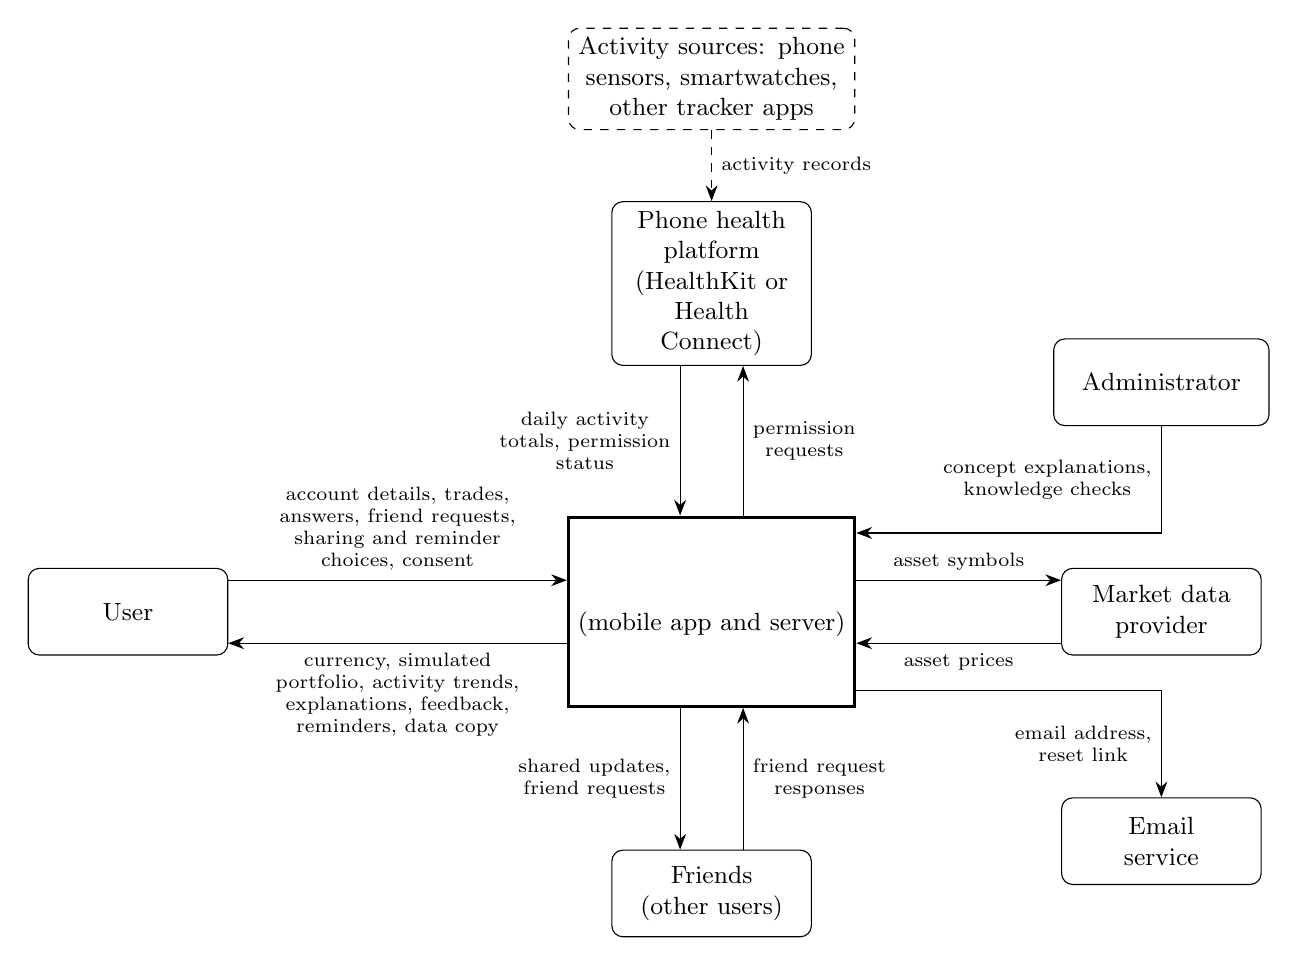
\begin{tikzpicture}[
  font=\small,
  entity/.style={draw, rounded corners, align=center, text width=2.3cm,
    minimum height=1.1cm},
  system/.style={draw, very thick, align=center, minimum width=3.2cm,
    minimum height=2.4cm, font=\large\bfseries},
  upstream/.style={draw, dashed, rounded corners, align=center,
    text width=3.4cm},
  flow/.style={-{Stealth[length=2mm]}},
  lbl/.style={font=\scriptsize, align=center}
]
  \node[system] (sys) {\progname{}\\[2pt]\normalfont\small (mobile app and server)};

  \node[entity, left=4.3cm of sys] (user) {User};
  \node[entity, right=2.6cm of sys] (market) {Market data\\provider};
  \node[entity, text width=2.5cm, above=1.8cm of market] (admin)
    {Administrator};
  \node[entity, below=1.8cm of market] (email) {Email\\service};
  \node[entity, above=1.9cm of sys] (health)
    {Phone health platform\\(HealthKit or\\Health Connect)};
  \node[entity, below=1.8cm of sys] (friends) {Friends\\(other users)};
  \node[upstream, above=0.9cm of health] (sources)
    {Activity sources: phone sensors, smartwatches, other tracker apps};

  % User
  \draw[flow] ([yshift=4mm]user.east) -- ([yshift=4mm]sys.west)
    node[lbl, midway, above] {account details, trades,\\answers, friend requests,\\sharing and reminder\\choices, consent};
  \draw[flow] ([yshift=-4mm]sys.west) -- ([yshift=-4mm]user.east)
    node[lbl, midway, below] {currency, simulated\\portfolio, activity trends,\\explanations, feedback,\\reminders, data copy};

  % Market data provider
  \draw[flow] ([yshift=4mm]sys.east) -- ([yshift=4mm]market.west)
    node[lbl, midway, above] {asset symbols};
  \draw[flow] ([yshift=-4mm]market.west) -- ([yshift=-4mm]sys.east)
    node[lbl, midway, below] {asset prices};

  % Health platform
  \draw[flow] ([xshift=-4mm]health.south) -- ([xshift=-4mm]sys.north)
    node[lbl, midway, left] {daily activity\\totals, permission\\status};
  \draw[flow] ([xshift=4mm]sys.north) -- ([xshift=4mm]health.south)
    node[lbl, midway, right] {permission\\requests};

  % Friends
  \draw[flow] ([xshift=-4mm]sys.south) -- ([xshift=-4mm]friends.north)
    node[lbl, midway, left] {shared updates,\\friend requests};
  \draw[flow] ([xshift=4mm]friends.north) -- ([xshift=4mm]sys.south)
    node[lbl, midway, right] {friend request\\responses};

  % Administrator
  \draw[flow] (admin.south) |- ([yshift=10mm]sys.east)
    node[lbl, pos=0.25, left] {concept explanations,\\knowledge checks};

  % Email service
  \draw[flow] ([yshift=-10mm]sys.east) -| (email.north)
    node[lbl, pos=0.75, left] {email address,\\reset link};

  % Activity sources (outside the system, never connected to it directly)
  \draw[flow, dashed] (sources.south) -- (health.north)
    node[lbl, midway, right] {activity records};
\end{tikzpicture}
\caption{System context of \progname{}}
\label{Fig_SystemContext}
\end{figure}

% Template prompt (hidden): List the responsibilities of each entity in the
% diagram, about inputs and outputs only, kept abstract but more specific than
% "inputs" and "outputs". The system should check data quality wherever
% possible; otherwise the user takes on that responsibility.

The responsibilities of each entity in Figure~\ref{Fig_SystemContext} are:

\begin{itemize}
\item User Responsibilities:
\begin{itemize}
\item Confirm truthfully that they are at least \texttt{MIN\_USER\_AGE} years
  old.
\item Keep any profile measurements they choose to enter, such as height and
  weight, accurate.
\item Grant \progname{} the permissions its features use, and keep an activity
  source recording to the phone's health platform.
\item Make their own trade decisions. \progname{} gives no financial advice.
\item Choose what to share, with which friends, and when to receive reminders.
\item Keep an Internet connection for trading and the social feed.
\item Keep their password private and keep access to their account's email
  address.
\end{itemize}
\item \progname{} Responsibilities:
\begin{itemize}
\item Reject profile measurements outside plausible ranges.
\item Award currency only for activity within plausibility limits and up to a
  daily cap (Hazard Analysis SAF-7, SEC-1).
\item Treat a day with no activity data as a day with zero activity.
\item Reject purchases that cost more than the user's balance and sales of
  more shares than the user holds (Hazard Analysis SEC-5).
\item Record each trade once and completely (Hazard Analysis SEC-5, SEC-6).
\item Show each asset price with the time it was obtained, and mark delayed
  prices (Hazard Analysis SEC-2).
\item Refuse trades on out-of-date prices while the market is open, and queue
  trades requested while it is closed (Hazard Analysis SEC-3, SEC-4).
\item Show each shared update only to the friends the user chose, without
  location detail (Hazard Analysis SEC-13, SEC-14).
\item Request only the permissions its features use, explaining each one
  (Hazard Analysis SEC-7, SEC-8).
\item Send the market data provider only the symbols of the assets being
  priced, and no personal or health data (Hazard Analysis SEC-11).
\item Send the email service no personal or health data other than the user's
  email address and their password reset link (Hazard Analysis SEC-11).
\end{itemize}
\item Health Platform Responsibilities:
\begin{itemize}
\item Store activity records from the user's activity sources, and provide
  daily totals for the activity types the user has permitted.
\item Grant or withdraw \progname{}'s read access as the user chooses, and
  report the current permission status.
\item Keep the activity data it records as accurate as its activity sources
  allow.
\end{itemize}
\item Market Data Provider Responsibilities:
\begin{itemize}
\item Supply current and historical prices for the assets \progname{}
  requests, within its request limits.
\end{itemize}
\item Email Service Responsibilities:
\begin{itemize}
\item Deliver each password reset link that \progname{} sends to the user's
  email address.
\end{itemize}
\item Administrator Responsibilities:
\begin{itemize}
\item Keep concept explanations and knowledge checks accurate, and name no
  asset for the user to buy or sell in them (Hazard Analysis SAF-9).
\end{itemize}
\item Friend Responsibilities:
\begin{itemize}
\item Accept or decline a user's friend request.
\item View the updates a user has shared with them in their social feed.
\end{itemize}
\end{itemize}

% Template prompts (hidden): Identify the context the software will typically
% be used in, and whether it will be used for mission-critical or
% safety-critical applications. This sets how much effort the rationale
% section needs.

\progname{} is intended for personal education and habit building. Members of
the general public use it on their own smartphones to track their activity,
earn currency and practice investing in a simulated market. It is not intended
for professional, engineering or scientific use.

\progname{} is not mission-critical: it holds and moves no real money, so an
outage only delays rewards and learning. It is not safety-critical either
since it controls no physical equipment and provides
no medical function. However, it handles personal health data and
is designed to influence how users exercise and make financial decisions. These
hazards, and the requirements that control them, are covered in the Hazard
Analysis. The rationale in Section~\ref{SecRationale} therefore focuses on
those requirements.

\subsection{User Characteristics} \label{SecUserCharacteristics}

% Template prompt (hidden): Summarize the knowledge and skills expected of the
% user, specifically and unambiguously. The user is a different role from the
% intended reader (Section 1.5). Usability requirements are measured against
% this typical user.

The typical user of \progname{} is a young adult, such as a student or someone
starting their first job (Problem Statement and Goals, Section~1). The user of
\progname{}:
\begin{itemize}
  \item Is at least \texttt{MIN\_USER\_AGE} years old (Hazard Analysis CA2).
  \item Uses a smartphone daily, and can install an app, grant or deny app
  permissions, and use common mobile app controls.
  \item Carries an Android or iOS phone during everyday activity. No wearable
  device or fitness expertise is required.
  \item Reads English, and has the numeracy of Grade~9 mathematics: working
  with percentages, comparing values, and reading a simple line chart.
  \item Needs no prior knowledge of investing terms such as stock,
  exchange-traded fund (ETF) or portfolio.
\end{itemize}

As per interviews conducted, participants mainly track their activity with a phone. Both
already knew some investing concepts, through self-study or formal study, and
both learned most by doing.
No one interviewed was a self-reported complete beginner, so the beginner characteristics above come
from the Problem Statement, and usability testing should include beginners.

\subsection{System Constraints}

% Template prompts (hidden): System constraints limit the developers' options
% in the design and identify how the system must fit into the world. This is
% the only place in the SRS where design decisions can be specified, so they
% should only be included if they are truly required. Mention platform
% constraints and licensing restrictions here.

The following constraints limit the design of \progname{}. Each one is imposed
by the project brief, an external service, the law or the app stores.

\begin{itemize}

\item[SC\refstepcounter{scnum}\thescnum \label{SC_Platform}:] \progname{} shall
run as a mobile app on Android phones running Android
\texttt{MIN\_ANDROID\_VERSION} or later and on iPhones running iOS
\texttt{MIN\_IOS\_VERSION} or later.
\textit{Rationale:} This project calls for a mobile app, and these are the
versions on the devices available to the team and the supervisor for testing
(Development Plan, Section~10).

\item[SC\refstepcounter{scnum}\thescnum \label{SC_HealthPlatform}:]
\progname{} shall obtain recorded activity only through the phone's health
platform: Apple HealthKit on iOS and Health Connect on Android. This rule also
covers any library \progname{} uses to read health data. No core feature shall
require a wearable device.
\textit{Rationale:} Users carry their phone during everyday activity
(Section~\ref{SecUserCharacteristics}), and the health platforms already
collect data from the phone and from any wearable the user owns (note, wearable
integration is a stretch goal).

\item[SC\refstepcounter{scnum}\thescnum \label{SC_HealthAccess}:] \progname{}
shall access health data only under the access rules Apple (iOS provider) and Google (Android OS provider) set for
their health platforms, such as declaring each data type it reads and
explaining each permission to the user \citep{AppleHealthKit,
GoogleHealthConnect}.
\textit{Rationale:} Apps that break these rules are not accepted in the app
stores. The rules also limit what \progname{} can read, such as how far back
past activity data can be read.

\item[SC\refstepcounter{scnum}\thescnum \label{SC_MarketData}:] \progname{}
shall obtain real-world asset prices from a third-party market data provider
(\texttt{MARKET\_DATA\_PROVIDER}), within the provider's request limits and
licence terms.
\textit{Rationale:} The team cannot produce market prices itself, so request
limits, cost and permitted use are set by the provider.

\item[SC\refstepcounter{scnum}\thescnum \label{SC_NoRealMoney}:] Virtual
currency and simulated holdings shall have no monetary value. They cannot be
bought with, redeemed for or exchanged for money, and \progname{} shall not
connect to any bank or brokerage account or give personalized investment
advice. \progname{} shall state the associated risks whenever it explains a financial concept.
\textit{Rationale:} Handling real money or giving personalized investment advice would bring
\progname{} under financial regulation that the team is not licensed for.
Keeping real money out also keeps the practice risk-free (G4).

\item[SC\refstepcounter{scnum}\thescnum \label{SC_Privacy}:] \progname{} shall
collect, use, store and delete personal and health data in line with
Canada's Personal Information Protection and Electronic Documents Act (PIPEDA)
and the health-data policies of the Apple App Store and Google Play.
\textit{Rationale:} These laws and policies apply to any app that handles this
data in Canada and in these stores. The specific controls are in
Section~\ref{SecPrivacyRetention} and the Hazard Analysis (SEC-7 to SEC-12 and
SEC-18).

\item[SC\refstepcounter{scnum}\thescnum \label{SC_Server}:] Trading, market
prices and the social feed shall require an Internet connection to
\progname{}'s server.
\textit{Rationale:} Prices are fetched from the provider once for all users to
stay within its request limits (\scref{SC_MarketData}), friends' shared updates
must reach other users' phones, and a user's portfolio must survive the loss of
their phone.

\end{itemize}




% ============================================================== 
\section{Stakeholder Requirements}

% \plt{Technology-independent requirements.  These come from statements made by
%   the stakeholders.  You will find these through interviews and surveys.  They are
%   often expressed in natural language.  They are not necessarily testable, but
%   they should be verifiable.}

% \plt{The stakeholder requirements are numbered so that you can have traceability to other parts of your document.}

% \noindent \begin{itemize}

%   \item[SR\refstepcounter{srnum}\thesrnum \label{SR_Label1}] TODO

%   \item[SR\refstepcounter{srnum}\thesrnum \label{SR_Label2}] TODO

%   \item[SR\refstepcounter{srnum}\thesrnum \label{SR_Label3}] TODO

% \end{itemize}

% \plt{You should give your SRs meaningful labels, so that you can refer to them
%   in other parts of the SRS.  The label names should be meaningful mnemonics, not
%   numbers.}


This section lists what the stakeholders in Table~\ref{TblStakeholders} need
from \progname{}, stated without reference to any technology. Each
requirement names its \emph{source} stakeholders, the \emph{evidence} for it,
and the product \emph{goal} from Section~2 that it supports. Use cases in
Section~5 and functional requirements in Section~6 refine these requirements
and trace back to them by their identifiers.

The evidence comes from three places. The Problem Statement and Goals document
records the client's vision and the target users. Two potential users were
interviewed on October~14, 2026, for the team's Design Thinking report; they
are referred to as P01 and P02, and their statements are paraphrased or
briefly quoted from de-identified transcripts. The Hazard Analysis contributes
needs that protect users from harm. Neither interviewee was a beginner at
investing, so the needs of beginners come from the Problem Statement and will
be checked in usability testing.

Each requirement is verifiable: it can be confirmed by inspection,
demonstration, or a usability test, through the functional and non-functional
requirements that refine it.

\paragraph{Activity and motivation}

{\sloppy
  \noindent\begin{itemize}
    \item[SR\refstepcounter{srnum}\thesrnum\label{SR_EarnFromActivity}:] Users shall be rewarded for the physical activity they already do, without having to start, stop, or record it themselves.\\
          \emph{Source:} SH1, SH2. \emph{Evidence:} Both participants track activity with their phone (P01, P02). Tracking should be ``as touchless as possible'': an app that must be started and stopped by hand is easily left running for hours and gives wrong results (P01). Approximate step counts are acceptable to users (P01). \emph{Goal:} G5.
    \item[SR\refstepcounter{srnum}\thesrnum\label{SR_UsefulRewards}:] Rewards for activity shall have a visible use to the user beyond the activity count itself.\\
          \emph{Source:} SH1, SH2. \emph{Evidence:} A long step streak gives one participant nothing but pride (P01); rewards have not changed the other's habits, although a tangible reward might make them work out more (P02). \emph{Goal:} G5.
    \item[SR\refstepcounter{srnum}\thesrnum\label{SR_AllAbilities}:] Users of any fitness level or physical ability shall be able to earn rewards, whatever kinds of activity they do.\\
          \emph{Source:} SH1, SH6. \emph{Evidence:} Participants' activity goes well beyond walking: basketball, skating, and pickup hockey (P01); soccer, weightlifting, climbing stairs, and rock climbing (P02). The target users have any level of fitness (Problem Statement). \emph{Goal:} G5.
    \item[SR\refstepcounter{srnum}\thesrnum\label{SR_OwnGoals}:] Users shall choose their own activity goals, or set none, and shall not be pressured to raise them.\\
          \emph{Source:} SH1. \emph{Evidence:} One participant has kept the same step goal for over a year, because a higher one takes too much time (P01); the other sets no goals and keeps only a mental check that they ``at least did something'' (P02). \emph{Goal:} G5.
    \item[SR\refstepcounter{srnum}\thesrnum\label{SR_SafeMotivation}:] Features that motivate activity shall not encourage users to exercise when it is unsafe, such as late at night, while injured, or beyond a healthy amount.\\
          \emph{Source:} SH1, SH6. \emph{Evidence:} A streak now makes one participant go out walking at 9~p.m.\ to reach their goal (P01); the other admires a friend for whom ``it doesn't matter how much anything hurts'' (P02). \emph{Goal:} G5.
  \end{itemize}
  \par}

\paragraph{Investing practice}

{\sloppy
  \noindent\begin{itemize}
    \item[SR\refstepcounter{srnum}\thesrnum\label{SR_RiskFree}:] Users shall be able to practise investing without any risk to real money.\\
          \emph{Source:} SH1, SH2. \emph{Evidence:} One participant was well-versed in financial math from university courses but did not know how to act on it until they started working with real investments (P02); the other first learned by tracking their own transactions by hand (P01). \emph{Goal:} G4.
    \item[SR\refstepcounter{srnum}\thesrnum\label{SR_RealMarket}:] Investing practice shall follow the real market closely enough that its lessons carry over to real investing.\\
          \emph{Source:} SH1, SH2. \emph{Evidence:} The client's vision is a portfolio that follows real-world prices (Problem Statement). \emph{Goal:} G4.
    \item[SR\refstepcounter{srnum}\thesrnum\label{SR_PastMarkets}:] Users shall be able to practise in past market conditions, such as a downturn, without affecting their own progress.\\
          \emph{Source:} SH1, SH2. \emph{Evidence:} Practising a downturn safely prepares users for one with real money (Problem Statement). \emph{Goal:} G4.
    \item[SR\refstepcounter{srnum}\thesrnum\label{SR_NotAdvice}:] \progname{} shall never give, or be mistaken for, advice on what to do with real money.\\
          \emph{Source:} SH1, SH6, SH9. \emph{Evidence:} Self-taught investors learn from YouTube and Reddit, where it is easy to follow ``the wrong kinds of investing YouTubers,'' and look for answers tailored to their own situation (P01). Users may act on whatever the app appears to recommend. \emph{Goal:} G4.
  \end{itemize}
  \par}

\paragraph{Learning}

{\sloppy
  \noindent\begin{itemize}
    \item[SR\refstepcounter{srnum}\thesrnum\label{SR_LearnInContext}:] Users shall be able to understand each financial and fitness concept where it appears, without leaving \progname{}.\\
          \emph{Source:} SH1. \emph{Evidence:} Beginners are told that investing requires studying measures such as price-to-earnings ratios, which confuses them (P01); advice is scattered across sources that contradict each other (Problem Statement). \emph{Goal:} G1, G2.
    \item[SR\refstepcounter{srnum}\thesrnum\label{SR_LearnByDoing}:] Users shall learn through activities they take part in, not only by reading or watching.\\
          \emph{Source:} SH1. \emph{Evidence:} One participant has trouble learning from videos and needs ``a component that's interactive''; watching alone ``doesn't stick'' (P02). The other learned investing by doing it themselves (P01). \emph{Goal:} G1.
    \item[SR\refstepcounter{srnum}\thesrnum\label{SR_LearnFromDecisions}:] Users shall be able to find out why their portfolio changed after their own decisions, including how diversified it is.\\
          \emph{Source:} SH1, SH2. \emph{Evidence:} One participant considers buying individual stocks ``almost like gambling'' compared with diversified index investing (P01); users need to see this in their own results. \emph{Goal:} G1.
    \item[SR\refstepcounter{srnum}\thesrnum\label{SR_CanadianContext}:] Users shall be able to learn how the concepts they practise apply to saving and investing in Canada, such as tax-free savings accounts.\\
          \emph{Source:} SH1, SH6. \emph{Evidence:} Both participants named Canada's account types, such as Tax-Free Savings Accounts (TFSAs) and Registered Retirement Savings Plans (RRSPs), as important things they had to learn (P01, P02); ``so many people aren't doing anything at all'' with their savings (P02). \emph{Goal:} G1.
    \item[SR\refstepcounter{srnum}\thesrnum\label{SR_SeeProgress}:] Users shall be able to see how their activity and their investments have changed over time, in one place.\\
          \emph{Source:} SH1. \emph{Evidence:} One participant checks their heart rate often, out of curiosity and to see that it is healthy (P02); the other tracks both their steps and their portfolio, in separate tools (P01). \emph{Goal:} G2.
  \end{itemize}
  \par}

\paragraph{Sharing and privacy}

{\sloppy
  \noindent\begin{itemize}
    \item[SR\refstepcounter{srnum}\thesrnum\label{SR_ShareProgress}:] Users shall be able to share the progress they choose with friends.\\
          \emph{Source:} SH1, SH5. \emph{Evidence:} Being ahead of friends ``feels great,'' and good friends help those who fall behind (P02). \emph{Goal:} G3.
    \item[SR\refstepcounter{srnum}\thesrnum\label{SR_ControlSharing}:] Users shall control exactly what their friends can see, and nothing shall be shared without the user's choice.\\
          \emph{Source:} SH1, SH5. \emph{Evidence:} Removing names does not make a person anonymous, because the stories they tell and other context can reveal who they are (P01). \emph{Goal:} G3.
    \item[SR\refstepcounter{srnum}\thesrnum\label{SR_NoHarmfulComparison}:] \progname{} shall not make users feel that they are falling far behind other users.\\
          \emph{Source:} SH1, SH6. \emph{Evidence:} Comparison is fine when slightly behind, and ``only ever bad when you're really far behind'' (P02). \emph{Goal:} G3.
    \item[SR\refstepcounter{srnum}\thesrnum\label{SR_ProtectData}:] Users' personal and health data shall be collected only where it is needed, kept secure, and never sold.\\
          \emph{Source:} SH1, SH9. \emph{Evidence:} One participant avoided step counters from large companies, turned off their step counter's network access, and keeps their portfolio records on their own computer (P01); the other shares data only with a reputable company that keeps it secure (P02). Required by PIPEDA~\citep{PIPEDA}. \emph{Goal:} G3.
    \item[SR\refstepcounter{srnum}\thesrnum\label{SR_ExplainPermissions}:] Users shall understand why each permission is needed before they grant it.\\
          \emph{Source:} SH1, SH7. \emph{Evidence:} Both participants grant a permission when there is a clear reason for it (P01, P02), and distrust apps that ask for ``12 permissions'' when two would do (P01). \emph{Goal:} G2, G3.
    \item[SR\refstepcounter{srnum}\thesrnum\label{SR_ControlOwnData}:] Users shall be able to withdraw their consent and delete their account and data.\\
          \emph{Source:} SH1, SH9. \emph{Evidence:} Users' right to withdraw consent is required by PIPEDA~\citep{PIPEDA}. \emph{Goal:} G3.
  \end{itemize}
  \par}

\paragraph{Access and operation}

{\sloppy
  \noindent\begin{itemize}
    \item[SR\refstepcounter{srnum}\thesrnum\label{SR_EasyStart}:] Users shall be able to install \progname{} from their phone's app store and start earning rewards without outside help.\\
          \emph{Source:} SH1, SH2. \emph{Evidence:} First-time users must complete the core tasks without outside help (Problem Statement Goal~2); how well an app is designed affects whether users trust it (P02). \emph{Goal:} G2.
    \item[SR\refstepcounter{srnum}\thesrnum\label{SR_PhoneOnly}:] Users shall be able to use every core feature with only their phone, on either Android or iOS, without a wearable device.\\
          \emph{Source:} SH1, SH2. \emph{Evidence:} One participant uses an Android phone and stopped wearing a fitness band because it irritated their skin (P01); the other uses an iPhone and an Apple Watch (P02). \emph{Goal:} G2, G5.
    \item[SR\refstepcounter{srnum}\thesrnum\label{SR_Accessible}:] Users with visual or motor disabilities shall be able to use the core features.\\
          \emph{Source:} SH1, SH6, SH9. \emph{Evidence:} Accessibility is part of serving every user and is expected by app stores (WCAG~2.2~\citep{WCAG22}). \emph{Goal:} G2.
    \item[SR\refstepcounter{srnum}\thesrnum\label{SR_UpdateContent}:] Administrators shall be able to update the tradable assets and the educational content without releasing a new version of the app.\\
          \emph{Source:} SH4. \emph{Evidence:} Educational content must be corrected and reviewed over time (Hazard Analysis), and the list of assets will change. \emph{Goal:} G1, G4.
    \item[SR\refstepcounter{srnum}\thesrnum\label{SR_RespectProviders}:] \progname{} shall use health and market data only within the terms and limits set by their providers.\\
          \emph{Source:} SH7, SH8. \emph{Evidence:} Providers limit what data can be read and how often prices can be requested (Problem Statement). \emph{Goal:} G4, G5.
  \end{itemize}
  \par}

Table~\ref{TblSHtoSR} traces each stakeholder requirement to the stakeholders
it comes from. Every stakeholder in Table~\ref{TblStakeholders} except the
development team (SH3), whose needs are expressed through the qualities of the
requirements themselves, is the source of at least one requirement.

\begin{table}[H]
  \caption{Traceability between stakeholders and stakeholder requirements}
  \label{TblSHtoSR}
  \small
  \centering
  \begin{tabular}{l*{9}{c}}
    \toprule
                                   & \multicolumn{9}{c}{\textbf{Stakeholder}}                                                                                                                         \\
    \cmidrule(l){2-10}
    \textbf{Requirement}           & \textbf{SH1}                             & \textbf{SH2} & \textbf{SH3} & \textbf{SH4} & \textbf{SH5} & \textbf{SH6} & \textbf{SH7} & \textbf{SH8} & \textbf{SH9} \\
    \midrule
    \srref{SR_EarnFromActivity}    & $\times$                                 & $\times$     &              &              &              &              &              &              &              \\
    \srref{SR_UsefulRewards}       & $\times$                                 & $\times$     &              &              &              &              &              &              &              \\
    \srref{SR_AllAbilities}        & $\times$                                 &              &              &              &              & $\times$     &              &              &              \\
    \srref{SR_OwnGoals}            & $\times$                                 &              &              &              &              &              &              &              &              \\
    \srref{SR_SafeMotivation}      & $\times$                                 &              &              &              &              & $\times$     &              &              &              \\
    \srref{SR_RiskFree}            & $\times$                                 & $\times$     &              &              &              &              &              &              &              \\
    \srref{SR_RealMarket}          & $\times$                                 & $\times$     &              &              &              &              &              &              &              \\
    \srref{SR_PastMarkets}         & $\times$                                 & $\times$     &              &              &              &              &              &              &              \\
    \srref{SR_NotAdvice}           & $\times$                                 &              &              &              &              & $\times$     &              &              & $\times$     \\
    \srref{SR_LearnInContext}      & $\times$                                 &              &              &              &              &              &              &              &              \\
    \srref{SR_LearnByDoing}        & $\times$                                 &              &              &              &              &              &              &              &              \\
    \srref{SR_LearnFromDecisions}  & $\times$                                 & $\times$     &              &              &              &              &              &              &              \\
    \srref{SR_CanadianContext}     & $\times$                                 &              &              &              &              & $\times$     &              &              &              \\
    \srref{SR_SeeProgress}         & $\times$                                 &              &              &              &              &              &              &              &              \\
    \srref{SR_ShareProgress}       & $\times$                                 &              &              &              & $\times$     &              &              &              &              \\
    \srref{SR_ControlSharing}      & $\times$                                 &              &              &              & $\times$     &              &              &              &              \\
    \srref{SR_NoHarmfulComparison} & $\times$                                 &              &              &              &              & $\times$     &              &              &              \\
    \srref{SR_ProtectData}         & $\times$                                 &              &              &              &              &              &              &              & $\times$     \\
    \srref{SR_ExplainPermissions}  & $\times$                                 &              &              &              &              &              & $\times$     &              &              \\
    \srref{SR_ControlOwnData}      & $\times$                                 &              &              &              &              &              &              &              & $\times$     \\
    \srref{SR_EasyStart}           & $\times$                                 & $\times$     &              &              &              &              &              &              &              \\
    \srref{SR_PhoneOnly}           & $\times$                                 & $\times$     &              &              &              &              &              &              &              \\
    \srref{SR_Accessible}          & $\times$                                 &              &              &              &              & $\times$     &              &              & $\times$     \\
    \srref{SR_UpdateContent}       &                                          &              &              & $\times$     &              &              &              &              &              \\
    \srref{SR_RespectProviders}    &                                          &              &              &              &              &              & $\times$     & $\times$     &              \\
    \bottomrule
  \end{tabular}
\end{table}
% ============================================================== 
\section{User Personas}
% \plt{Create 2-5 realistic personas.
%   Personas are fictional characters that represent the different user types that
%   might use your software.  They are used to help understand the users'
%   needs, experiences, behaviors and goals.  They are not real people, but they
%   should be based on real data collected from user research.}

The personas below represent the main kinds of user \progname{} is built for.
They are fictional, but each is based on the evidence named in its
\emph{Based on} entry: Personas~1 and~2 on the two interviews (P01 and P02),
and Persona~3 on the target users in the Problem Statement, since neither
interviewee was a beginner at investing. Details that could identify an
interviewee have been changed. Each persona lists the stakeholder requirements
that matter most to them, so the design can be checked against the people it
serves.

\subsection{Persona 1}
\begin{itemize}
  \item \textbf{Name:} Sam, 28, graduate student.
  \item \textbf{Description:} Walks to campus and back every day and has tracked
        steps on an Android phone for years. A streak of more than a year at a
        fixed step goal now gets Sam out walking at 9~p.m.\ on slow days, although
        Sam has never raised the goal. Sam also plays pickup sports and skates in
        winter, none of which is tracked, and stopped wearing a fitness band because
        it irritated their skin. Sam taught themselves investing from videos, online
        forums, and books, and prefers simple, diversified index investing.
  \item \textbf{Goals:} Keep the streak going without it taking over the
        evening; get credit for sports, not only steps; keep learning investing in a
        way that fits their own situation; keep control of their data.
  \item \textbf{Frustrations:} Apps that must be started and stopped by hand;
        investing content that pushes risky stock-picking; apps that ask for far more
        permissions than they need or that may sell their data.
  \item \textbf{Technical Ability:} High. Sam chooses apps for privacy, turns off
        an app's network access, and keeps financial records on their own computer.
  \item \textbf{Based on:} P01.
  \item \textbf{Most relevant requirements:} \srref{SR_EarnFromActivity},
        \srref{SR_AllAbilities}, \srref{SR_SafeMotivation}, \srref{SR_NotAdvice},
        \srref{SR_ProtectData}, \srref{SR_ExplainPermissions}, \srref{SR_PhoneOnly}.
\end{itemize}

\subsection{Persona 2}
\begin{itemize}
  \item \textbf{Name:} Jordan, 24, early-career employee in financial services.
  \item \textbf{Description:} Took several finance courses at university, but
        only understood how to act on them once their job involved real investments.
        Walks, lifts weights now and then, and enjoys rock climbing; used to play
        soccer. Exercise is not a priority right now. Jordan's iPhone counts their
        steps and the stairs they climb, and they often check their heart rate on an
        Apple Watch out of curiosity. Jordan sets no fitness goals and keeps only a
        mental note of whether they did something that week.
  \item \textbf{Goals:} Be more consistent with exercise, like a friend Jordan
        admires; learn by doing rather than by watching; understand their account
        options well enough that their savings grow instead of falling behind
        inflation.
  \item \textbf{Frustrations:} Learning from videos that do not stick;
        falling far behind friends; apps that ask for personal data without a clear
        reason.
  \item \textbf{Technical Ability:} Moderate to high. Uses a phone and smartwatch
        daily, and judges whether to trust an app by who makes it and how well it is
        designed.
  \item \textbf{Based on:} P02.
  \item \textbf{Most relevant requirements:} \srref{SR_UsefulRewards},
        \srref{SR_LearnByDoing}, \srref{SR_CanadianContext},
        \srref{SR_ShareProgress}, \srref{SR_NoHarmfulComparison},
        \srref{SR_OwnGoals}, \srref{SR_ExplainPermissions}.
\end{itemize}


\subsection{Persona 3}
\begin{itemize}
  \item \textbf{Name:} Aisha, 19, first-year student.
  \item \textbf{Description:} Has never invested and does not know what a stock,
        an exchange-traded fund, or a tax-free savings account is. Her savings sit in
        a bank account. She walks between classes but does not exercise regularly.
        She would like to start investing, but is afraid of losing money she cannot
        afford to lose and has heard that investing means studying company finances.
  \item \textbf{Goals:} Understand the basics of investing in plain language;
        start a fitness habit without being judged; try things without real
        consequences.
  \item \textbf{Frustrations:} Financial jargon; advice that contradicts other
        advice; apps that assume she already knows how they work.
  \item \textbf{Technical Ability:} Everyday smartphone use: she can install an
        app and respond to permission prompts, but has never used a fitness or
        investing app.
  \item \textbf{Based on:} the target users described in the Problem Statement,
        and both interviewees' observations that many people do nothing with their
        savings (P02) and that beginners are put off by the belief that investing
        requires expert analysis (P01). This persona will be validated in usability
        testing.
  \item \textbf{Most relevant requirements:} \srref{SR_RiskFree},
        \srref{SR_LearnInContext}, \srref{SR_CanadianContext}, \srref{SR_EasyStart},
        \srref{SR_AllAbilities}, \srref{SR_SeeProgress}.
\end{itemize}

% ============================================================== 
\section{Use Cases}
\plt{Use cases are a way to describe the interactions between users and the system.
  They are typically written in natural language and describe the steps that a
  user takes to achieve a specific goal.  Use cases can be used to identify
  functional requirements and to create test cases.}
\plt{Typically 8-15 substantial use cases.}

\refstepcounter{ucnum} \label{UC_Label1}
\subsection{\ucref{UC_Label1}: Example Use Case}

\textbf{Primary Actor}

TODO

\textbf{Preconditions}
\begin{itemize}
  \item TODO
\end{itemize}

\textbf{Main Success Scenario}
\begin{enumerate}
  \item TODO
  \item TODO
  \item TODO
\end{enumerate}

\textbf{Alternative Flows}
\begin{itemize}
  \item TODO
\end{itemize}

\textbf{Postconditions}
\begin{itemize}
  \item TODO
\end{itemize}

% ============================================================== 
\section{Functional Requirements} \label{SecFR}

% Template prompts (hidden): Functional requirements describe what the system
% should do, derived from the stakeholder requirements and use cases. Use SHALL
% statements. Requirements must be atomic, testable and traceable. Labels are
% meaningful mnemonics, not numbers.

% =============================================================================
% HOW TO WRITE A FUNCTIONAL REQUIREMENT (delete this block before submitting)
%
% * Use \freq{label}{statement}{fit criterion}{traces}. The FR number is
%   assigned automatically.
% * Labels: FR_ plus the area prefix of your subsection, then a short name:
%   FR_Acct..., FR_Act..., FR_Mkt..., FR_Learn..., FR_Social..., and FR_Remind...
%   or FR_Set... in Reminders and Settings.
%   The prefix keeps labels from clashing between authors.
% * Statement: one "The system shall ..." per requirement. If it needs "and" to
%   join two behaviours, split it into two requirements.
% * Say WHAT, not how: no screens, libraries or algorithms. Numbers are
%   SMALL_CAPS constants defined in Appendix C (#95).
% * Fit criterion: one line saying how a tester decides pass or fail.
% * Traces to, in this order: stakeholder requirement(s) (\srref{SR_...},
%   Section 3, #127), use case(s) (\ucref{UC_...}, Section 5, #130), goal(s)
%   G1-G5 (Section 2.2), then any HA ID. SR and UC refs print as ?? until those
%   PRs merge. Leave out the SR or UC when none fits.
% * Hazard Analysis requirements that are functional (SAF-1 to SAF-11, SEC-1
%   to SEC-6) go here with their HA ID at the start of the statement, e.g.
%   "(HA SAF-1) The system shall ...", with the same statement and fit
%   criterion as the Hazard Analysis. Privacy and security requirements
%   (SEC-7 to SEC-18) go in Section 7.3 or Section 8 instead.
% * A requirement that implements part of an HA requirement without restating
%   it ends its Traces to with the HA ID, e.g. "G3, Hazard Analysis SEC-13".
% * Each subsection has one owner (in its comment).
% =============================================================================

This section lists what \progname{} shall do, grouped by feature area. Each
requirement has a fit criterion and traces to the stakeholder requirements and
use cases it refines and to the goals in Section~\ref{SecProductVision}. A
requirement that begins with a Hazard Analysis (HA) identifier, such as
(HA SEC-3), appears in the Hazard Analysis with the same identifier and
wording. A requirement whose traces end with a Hazard Analysis identifier, such
as Hazard Analysis SEC-13, implements part of that Hazard Analysis
requirement.

% Owner: Farid
\subsection{Accounts and Profile}

\noindent \begin{itemize}
\freq{FR_AcctCreate}
  {The system shall let a new user create an account with an email address and
  a password.}
  {A test user who enters an unused email address and a valid password has an
  account, and can sign in with them.}
  {\srref{SR_EasyStart}, G2}
\freq{FR_AcctAgeConfirm}
  {The system shall not create an account until the user confirms that they are
  at least \texttt{MIN\_USER\_AGE} years old.}
  {A test user who does not confirm their age during sign-up has no account
  created.}
  {\srref{SR_ProtectData}, G3, Hazard Analysis CA2}
\freq{FR_AcctUsername}
  {The system shall require each user to choose a username that no other user
  has.}
  {A test user who tries to sign up with a username that another account
  already uses is asked to choose a different one.}
  {\srref{SR_ShareProgress}, G3}
\freq{FR_AcctSignIn}
  {The system shall let a user sign in with their email address and password.}
  {A test user who enters their correct email address and password is signed
  in; one who enters a wrong password is not.}
  {\srref{SR_ProtectData}, G2}
\freq{FR_AcctSignOut}
  {The system shall let a signed-in user sign out.}
  {After a test user signs out, opening the app shows the sign-in screen and
  none of their data.}
  {\srref{SR_ProtectData}, G3}
\freq{FR_AcctResetPassword}
  {The system shall let a user who has forgotten their password set a new one
  through a link sent to their account's email address.}
  {A test user who requests a reset receives a link at their email address,
  and after setting a new password can sign in only with the new one.}
  {\srref{SR_ControlOwnData}, G2}
\freq{FR_AcctEditProfile}
  {The system shall let the user view and edit their profile details.}
  {A test user who changes a profile detail sees the new value the next time
  they open their profile.}
  {\srref{SR_ControlOwnData}, G3}
\freq{FR_AcctBodyOptional}
  {The system shall not require the user to enter their height or weight in
  order to use any feature.}
  {A test user who leaves height and weight empty can earn currency, trade,
  learn, and share.}
  {\srref{SR_AllAbilities}, \srref{SR_ProtectData}, G3, G5}
\freq{FR_AcctDownloadData}
  {The system shall let the user download a copy of the personal data
  \progname{} stores about them.}
  {A test user who requests a copy receives a file containing their profile,
  activity totals, balance, holdings, trades, and shared updates.}
  {\srref{SR_ControlOwnData}, G3}
\freq{FR_AcctDeleteConfirm}
  {Before deleting an account, the system shall ask the user to confirm the
  deletion in a message stating that it cannot be undone.}
  {A test user who starts account deletion is shown this warning, and their
  account still exists if they cancel.}
  {\srref{SR_ControlOwnData}, \ucref{UC_DeleteAccount}, G3}
\freq{FR_AcctDelete}
  {The system shall let the user delete their account from within the app.}
  {A test user who confirms deletion can no longer sign in, and none of their
  data is shown to them or to their friends.}
  {\srref{SR_ControlOwnData}, \ucref{UC_DeleteAccount}, G3, Hazard Analysis
  SEC-18}
\end{itemize}

% Owner: Davis
\subsection{Activity and Rewards}

\noindent \begin{itemize}
\freq{FR_ActTypes}
  {The system shall award virtual currency for at least
  \texttt{MIN\_ACTIVITY\_TYPES} activity types (the supported activity types).}
  {A tester records activity of \texttt{MIN\_ACTIVITY\_TYPES} different activity
  types in the health platform, and each one earns currency.}
  {\srref{SR_AllAbilities}, \ucref{UC_EarnCurrency}, G5}
\freq{FR_ActEarn}
  {The system shall award virtual currency for recorded activity of a supported
  activity type.}
  {For a test user whose recorded activity in one calendar day is plausible and
  would earn at most \texttt{MAX\_DAILY\_CURRENCY}, the balance increases by the sum, over the
  supported activity types, of each type's daily total multiplied by its rate
  in \texttt{EARNING\_RATES}.}
  {\srref{SR_EarnFromActivity}, \ucref{UC_EarnCurrency}, G5}
\freq{FR_ActNoData}
  {The system shall treat a day with no activity data from the health platform
  as a day with zero activity.}
  {For a test user whose health platform reports no activity data for a day,
  that day shows zero activity and earns no currency.}
  {\srref{SR_EarnFromActivity}, \ucref{UC_EarnCurrency}, G5}
\freq{FR_ActPlausible}
  {(HA SEC-1) The system shall not count an activity record that exceeds the
  plausibility limits for its activity type toward the user's currency,
  activity trends, streak or milestones, and shall show the user that the
  record was not counted.}
  {A test record of more than \texttt{MAX\_DAILY\_STEPS} steps in one day, or
  a workout longer than \texttt{MAX\_WORKOUT\_DURATION}, earns no currency,
  does not appear in the user's activity trends, streak or milestones, and is
  shown to the user as not counted.}
  {\srref{SR_EarnFromActivity}, \ucref{UC_EarnCurrency}, G5}
\freq{FR_ActDailyCap}
  {(HA SAF-7) The system shall award a user no more than
  \texttt{MAX\_DAILY\_CURRENCY} virtual currency for recorded activity in any
  calendar day.}
  {For a test user whose recorded activity in one calendar day is plausible and
  would otherwise earn more than \texttt{MAX\_DAILY\_CURRENCY}, the balance increases by exactly
  \texttt{MAX\_DAILY\_CURRENCY} for that day. Each activity counts toward the
  calendar day in the user's time zone at the time of the activity.}
  {\srref{SR_SafeMotivation}, \ucref{UC_EarnCurrency}, G5}
\freq{FR_ActGoal}
  {The system shall let the user set or change a daily activity goal for a
  supported activity type, with each change applying from the next day.}
  {A test user who changes their daily activity goal keeps the previous goal
  for the rest of that day and has the new goal from the next day.}
  {\srref{SR_OwnGoals}, G5}
\freq{FR_ActGoalOptional}
  {(HA SAF-3) The system shall not require the user to set an activity goal in
  order to earn currency for recorded activity.}
  {A test user with no activity goal set who records activity receives
  currency for it.}
  {\srref{SR_OwnGoals}, \ucref{UC_EarnCurrency}, G5}
\freq{FR_ActNoAutoGoal}
  {(HA SAF-4) The system shall not change a user's activity goal without the
  user's confirmation.}
  {A test user who exceeds their goal on \texttt{GOAL\_REVIEW\_PERIOD}
  consecutive days still has the same goal unless they confirm a change.}
  {\srref{SR_OwnGoals}, G5}
\freq{FR_ActStreak}
  {The system shall show the user their current streak.}
  {A test user with no streak who meets their activity goal on three
  consecutive days is shown a streak of 3. After a following rest day, they
  are shown a streak of 4. After a following day on which they neither
  meet their goal nor take a rest day, they are shown a streak of 0.}
  {\srref{SR_SeeProgress}, G5}
\freq{FR_ActRestDay}
  {(HA SAF-1) The system shall let the user mark up to
  \texttt{REST\_DAYS\_PER\_PERIOD} days in each \texttt{STREAK\_PERIOD} as
  rest days, and a rest day shall not end the user's activity streak.}
  {A test user with a streak who marks a day as a rest day and records no
  activity that day does not have the streak reset to zero at the start of the
  following day. A request to mark more than \texttt{REST\_DAYS\_PER\_PERIOD}
  rest days in one \texttt{STREAK\_PERIOD} is refused.}
  {\srref{SR_SafeMotivation}, G5}
\freq{FR_ActNoPenalty}
  {(HA SAF-2) The system shall not reduce a user's virtual currency balance or
  simulated holdings when they miss an activity goal or their streak ends, and
  shall not show a missed goal or an ended streak to other users.}
  {For a test user who misses their goal on day \textit{d}, the currency
  balance and simulated holdings at the start of day \textit{d+1} equal those
  at the end of day \textit{d}. No friend's social feed shows the missed goal
  or the ended streak.}
  {\srref{SR_SafeMotivation}, \srref{SR_NoHarmfulComparison}, G3, G5}
\freq{FR_ActMilestone}
  {The system shall show the user each milestone in \texttt{MILESTONES} when
  they reach it.}
  {A test user whose streak, or total currency earned, first reaches a value in
  \texttt{MILESTONES} is shown that milestone once.}
  {\srref{SR_SeeProgress}, G5}
\freq{FR_ActTrends}
  {The system shall show the user their daily totals for each supported
  activity type over time.}
  {A test user with recorded activity on 14 days sees the total for each of
  those days, for each supported activity type.}
  {\srref{SR_SeeProgress}, G2, G5}
\end{itemize}

% Owner: Davis
\subsection{Simulated Market and Portfolio}

\noindent \begin{itemize}
\freq{FR_MktAssetCount}
  {The system shall offer at least \texttt{MIN\_TRADABLE\_ASSETS} assets for
  trading in the simulated market.}
  {A tester counts the assets that can be traded in the simulated market and
  finds at least \texttt{MIN\_TRADABLE\_ASSETS}.}
  {\srref{SR_RealMarket}, \ucref{UC_ViewMarket}, G4}
\freq{FR_MktRealPrices}
  {The system shall price each asset in the simulated market at the most recent
  price it has obtained for that asset from the market data provider.}
  {For a test asset, the price \progname{} shows and uses for trades equals the
  latest price \progname{} received from the market data provider for that
  asset.}
  {\srref{SR_RealMarket}, \ucref{UC_ViewMarket}, G4}
\freq{FR_MktPriceAge}
  {(HA SEC-2) The system shall display each asset price with the time it was
  obtained, and shall mark the price as delayed when it is older than
  \texttt{QUOTE\_STALENESS\_LIMIT}.}
  {A test price obtained more than \texttt{QUOTE\_STALENESS\_LIMIT} ago is shown
  with its time and a ``Delayed'' marker. A price obtained within the limit is
  shown with its time and no marker.}
  {\srref{SR_RealMarket}, \ucref{UC_ViewMarket}, G4}
\freq{FR_MktSimNotice}
  {(HA SAF-8) Before the user's first trade, the system shall display a notice
  stating that the market is simulated, that virtual currency and holdings
  have no real-world value, and that nothing in \progname{} is financial
  advice. The system shall not complete the first trade until the user
  acknowledges the notice.}
  {A new test user who attempts their first trade is shown the notice and
  cannot complete the trade until they acknowledge it. The notice contains all
  three statements: the market is simulated, currency and holdings have no
  real-world value, and nothing in \progname{} is financial advice.}
  {\srref{SR_NotAdvice}, \ucref{UC_BuyAsset}, G4}
\freq{FR_MktBuy}
  {The system shall let the user buy shares of an asset using virtual currency.}
  {While a test asset's market is open, a test user with enough currency buys
  one share of it. Their balance decreases by the price shown when they
  confirmed the trade, and their holding of it increases by one.}
  {\srref{SR_RiskFree}, \srref{SR_LearnByDoing}, \ucref{UC_BuyAsset}, G4}
\freq{FR_MktSell}
  {The system shall let the user sell shares of an asset they hold for virtual
  currency.}
  {While a test asset's market is open, a test user holding one share of it
  sells it. Their balance increases by the price shown when they confirmed the
  trade, and their holding of it decreases by one.}
  {\srref{SR_RiskFree}, \srref{SR_LearnByDoing}, G4}
\freq{FR_MktAtomicTrade}
  {(HA SEC-5) The system shall record each trade completely, updating both the
  currency balance and the holdings, or not at all. It shall reject a purchase
  that costs more than the user's currency balance and a sale of more shares
  than the user holds.}
  {A test trade interrupted before it completes leaves the balance and
  holdings unchanged, and a completed trade changes both. A purchase costing
  more than the balance, or a sale of more shares than are held, is rejected
  and changes neither.}
  {\srref{SR_RealMarket}, \ucref{UC_BuyAsset}, G4}
\freq{FR_MktNoDuplicate}
  {(HA SEC-6) The system shall record a trade only once when the same trade
  request is submitted more than once.}
  {When a test user submits a trade and the same request is sent again, for
  example by retrying after a dropped connection, exactly one trade is
  recorded.}
  {\srref{SR_RealMarket}, \ucref{UC_BuyAsset}, G4}
\freq{FR_MktNoStaleTrade}
  {(HA SEC-3) The system shall not execute a trade while the asset's market is
  open and the asset's price is older than \texttt{QUOTE\_STALENESS\_LIMIT}.}
  {While a test asset's market is open and its price is older than
  \texttt{QUOTE\_STALENESS\_LIMIT}, a trade request for it is refused and the
  user is told the price is out of date. With a price within the limit, the
  trade proceeds.}
  {\srref{SR_RealMarket}, \ucref{UC_BuyAsset}, G4}
\freq{FR_MktQueueClosed}
  {(HA SEC-4) The system shall queue a trade requested while the asset's market
  is closed, and execute it at the first price obtained after the market next
  opens.}
  {A test trade requested while the market is closed is shown to the user as
  queued, with a notice that it will run at the opening price, and is executed
  at the first price obtained after the market opens.}
  {\srref{SR_RealMarket}, \ucref{UC_BuyAsset}, G4}
\freq{FR_MktHoldings}
  {The system shall show the user each of their holdings.}
  {A test user who owns shares of two assets sees both holdings, each with the
  number of shares held.}
  {\srref{SR_SeeProgress}, \ucref{UC_InvestmentFeedback}, G2, G4}
\freq{FR_MktPortfolioValue}
  {The system shall show the user their portfolio value.}
  {For a test user with known holdings, the portfolio value shown equals the
  sum of each holding multiplied by its asset's most recent price.}
  {\srref{SR_SeeProgress}, \ucref{UC_InvestmentFeedback}, G2, G4}
\freq{FR_MktLabelReturns}
  {(HA SAF-10) The system shall label every displayed return and portfolio
  value as simulated.}
  {Every screen that shows a return or portfolio value shows a ``Simulated''
  label next to it.}
  {\srref{SR_NotAdvice}, \ucref{UC_InvestmentFeedback}, G4}
\freq{FR_MktNoRecommend}
  {(HA SAF-9) The system shall not recommend that a user buy or sell a
  specific asset.}
  {No screen or notification shown to a test user tells them to buy or sell a
  named asset, or presents assets as a ``recommended pick''.}
  {\srref{SR_NotAdvice}, \ucref{UC_InvestmentFeedback}, G1, G4}
\end{itemize}

% Owner: Farid
\subsection{Learning and Feedback}

The requirements in this subsection refer to the core concepts in
Table~\ref{TblCoreConcepts}. These are the concepts measured by the knowledge
check in goal G1; the list is educational content that administrators can
extend without changing these requirements.

\begin{table}[H]
\caption{Core concepts} \label{TblCoreConcepts}
\small
\begin{tabularx}{\textwidth}{>{\raggedright\arraybackslash}p{0.18\textwidth}X}
\toprule
\textbf{Domain} & \textbf{Core concepts}\\
\midrule
Investing & Stock; ETF; share; market price; portfolio value; return;
diversification; risk and volatility; compound growth; market downturn and
recovery\\
Canadian accounts & Tax-Free Savings Account (TFSA); Registered Retirement
Savings Plan (RRSP)\\
Fitness & Each supported activity type; active minutes; rest day;
streak\\
\bottomrule
\end{tabularx}
\end{table}

\noindent \begin{itemize}
\freq{FR_LearnExplainConcept}
  {The system shall provide a concept explanation for each core concept in
  Table~\ref{TblCoreConcepts}.}
  {For every core concept in Table~\ref{TblCoreConcepts}, a tester can open a
  concept explanation of it in the app.}
  {\srref{SR_LearnInContext}, \srref{SR_CanadianContext}, G1}
\freq{FR_LearnInPlace}
  {The system shall let the user open the concept explanation of a core concept
  from every screen on which that concept appears.}
  {On every screen that shows a core concept, a tester can open its concept
  explanation without leaving that screen.}
  {\srref{SR_LearnInContext}, G1, G2}
\freq{FR_LearnValueChange}
  {When the user's portfolio value has changed by more than
  \texttt{FEEDBACK\_THRESHOLD} since they last viewed their portfolio,
  the system shall show feedback naming the holdings that contributed most to
  the change.}
  {For a test portfolio whose value has changed by more than the threshold,
  the feedback names the holding whose value changed most.}
  {\srref{SR_LearnFromDecisions}, G1}
\freq{FR_LearnTradeEffect}
  {After each trade, the system shall show the user how the trade changed the
  share of their portfolio value held in each asset.}
  {After a test trade, the feedback shows each holding's share of portfolio
  value before and after the trade, and these match the values calculated from
  the holdings.}
  {\srref{SR_LearnByDoing}, \srref{SR_LearnFromDecisions}, G1, G4}
\freq{FR_LearnConcentration}
  {When a single holding is more than \texttt{CONCENTRATION\_LIMIT} of the
  user's portfolio value, the system shall show the user an explanation of
  diversification.}
  {A test portfolio with one holding above \texttt{CONCENTRATION\_LIMIT} of its
  value shows the explanation, and the explanation names no asset to buy or
  sell (Hazard Analysis SAF-9).}
  {\srref{SR_LearnFromDecisions}, \srref{SR_NotAdvice}, G1, Hazard Analysis
  SAF-9}
\freq{FR_LearnKnowledgeCheck}
  {The system shall provide a knowledge check for each core concept in
  Table~\ref{TblCoreConcepts}.}
  {For every core concept in Table~\ref{TblCoreConcepts}, a tester can start a
  knowledge check on it.}
  {\srref{SR_LearnByDoing}, G1}
\freq{FR_LearnCheckResult}
  {When the user finishes a knowledge check, the system shall show which of
  their answers were correct and an explanation of the correct answer to each
  question they got wrong.}
  {A test user who answers one question wrongly sees that question marked
  incorrect, together with the explanation of its correct answer.}
  {\srref{SR_LearnFromDecisions}, G1}
\freq{FR_LearnProgress}
  {The system shall show the user their learning progress.}
  {After a test user views a concept explanation and passes a knowledge check,
  both appear in their learning progress.}
  {\srref{SR_SeeProgress}, G1, G2}
\freq{FR_LearnUpdateContent}
  {The system shall let administrators add and edit concept explanations and
  knowledge checks without releasing a new version of the app.}
  {A concept explanation edited by an administrator is shown in its edited form
  on a test phone whose app has not been updated.}
  {\srref{SR_UpdateContent}, G1}
\end{itemize}

% Owner: Farid
\subsection{Social Feed}

A user can share only the kinds of update in Table~\ref{TblShareable}. Currency
balances and portfolio values are not shareable, so that friends compare
effort and learning rather than market results.

\begin{table}[H]
\caption{Kinds of shared update} \label{TblShareable}
\small
\begin{tabularx}{\textwidth}{>{\raggedright\arraybackslash}p{0.28\textwidth}X}
\toprule
\textbf{Kind} & \textbf{Content}\\
\midrule
Activity total & The user's total for one activity type over a day or a
week\\
Streak & The user's current streak, in days. A rest day does not end a
streak (Hazard Analysis SAF-1)\\
Fitness milestone & A fitness milestone the user has reached\\
Learning milestone & A knowledge check the user has passed\\
\bottomrule
\end{tabularx}
\end{table}

\noindent \begin{itemize}
\freq{FR_SocialRequest}
  {The system shall let the user send a friend request to another user by
  their username.}
  {A test user who enters another user's username sends that user a friend
  request, which the other user sees.}
  {\srref{SR_ShareProgress}, \ucref{UC_ShareProgress}, G3}
\freq{FR_SocialAccept}
  {The system shall make two users friends only after the user who received
  the friend request accepts it.}
  {Two test users are not friends while a request between them is pending or
  after it is declined, and are friends once it is accepted.}
  {\srref{SR_ControlSharing}, G3}
\freq{FR_SocialDecline}
  {The system shall let the user decline a friend request.}
  {After a test user declines a request, the two users are not friends and the
  request is no longer shown to the user who declined it.}
  {\srref{SR_ControlSharing}, G3}
\freq{FR_SocialRemove}
  {The system shall let the user remove a friend.}
  {After a test user removes a friend, neither user sees the other's shared
  updates.}
  {\srref{SR_ControlSharing}, G3, Hazard Analysis SEC-13}
\freq{FR_SocialShare}
  {The system shall let the user share an update of a kind listed in
  Table~\ref{TblShareable}.}
  {A test user can share one update of each kind in Table~\ref{TblShareable},
  and cannot share anything else.}
  {\srref{SR_ShareProgress}, \ucref{UC_ShareProgress}, G3}
\freq{FR_SocialChooseFriends}
  {The system shall let the user choose which of their friends can see each
  shared update.}
  {A test update shared with one selected friend appears in that friend's
  social feed and in no other friend's.}
  {\srref{SR_ControlSharing}, \ucref{UC_ShareProgress}, G3, Hazard Analysis
  SEC-13}
\freq{FR_SocialPreview}
  {The system shall share an update only after showing the user the update
  exactly as their friends will see it.}
  {For every test update, the preview shown before sharing matches what the
  selected friends see in their social feed.}
  {\srref{SR_ControlSharing}, \ucref{UC_ShareProgress}, G3}
\freq{FR_SocialNoBody}
  {The system shall not include the user's age, height, or weight in any
  shared update.}
  {No shared update shown to a test user's friends contains their age, height,
  or weight.}
  {\srref{SR_ProtectData}, G3}
\freq{FR_SocialFeed}
  {The system shall show the user a social feed of the updates their friends
  have shared with them, newest first.}
  {A test user's social feed contains every update shared with them by a friend
  and no others, ordered by the time each was shared.}
  {\srref{SR_ShareProgress}, G3}
\freq{FR_SocialDeleteUpdate}
  {The system shall let the user delete an update they have shared.}
  {After a test user deletes a shared update, it no longer appears in any
  friend's social feed.}
  {\srref{SR_ControlSharing}, G3, Hazard Analysis SEC-13}
\freq{FR_SocialNoRanking}
  {(HA SAF-11) The system shall not rank users against each other by activity,
  currency or portfolio performance.}
  {No screen shown to a test user orders users by activity, currency or
  portfolio performance, or shows a user's position relative to others.}
  {\srref{SR_NoHarmfulComparison}, G3}
\end{itemize}

% Owner: Davis
\subsection{Reminders and Settings}

\progname{} sends reminders of the types in Table~\ref{TblReminderTypes}, which
are the same reminder types as in the Hazard Analysis.

\begin{table}[H]
\caption{Reminder types} \label{TblReminderTypes}
\small
\begin{tabularx}{\textwidth}{>{\raggedright\arraybackslash}p{0.14\textwidth}X>{\raggedright\arraybackslash}p{0.3\textwidth}}
\toprule
\textbf{Type} & \textbf{Example} & \textbf{Feature area}\\
\midrule
Activity & Progress toward today's goal, or a streak about to end & Activity and Rewards\\
Milestone & A goal reached, or a streak or currency milestone & Activity and Rewards\\
Portfolio & A notable change in simulated portfolio value & Simulated Market and Portfolio\\
Learning & A new concept explanation or knowledge check is available & Learning and Feedback\\
Social & A friend shared an update or sent a friend request & Social Feed\\
\bottomrule
\end{tabularx}
\end{table}

\noindent \begin{itemize}
\freq{FR_RemindPeriods}
  {The system shall let the user choose the time periods in which they receive
  reminders.}
  {A test user sets a reminder period, and it is shown in their settings the
  next time they open the app.}
  {\srref{SR_SafeMotivation}, \ucref{UC_Reminders}, G2, Hazard Analysis SAF-6}
\freq{FR_RemindInPeriods}
  {(HA SAF-6) The system shall send reminders of the types in
  Table~\ref{TblReminderTypes} only during the time periods the user has chosen
  to receive them.}
  {For a test user who has chosen their reminder periods, no reminder of any type
  in Table~\ref{TblReminderTypes} is delivered outside those periods. For a test
  user who has not chosen any periods, reminders are delivered only during
  \texttt{DEFAULT\_REMINDER\_PERIOD}.}
  {\srref{SR_SafeMotivation}, \ucref{UC_Reminders}, G2}
\freq{FR_SetWithdrawConsent}
  {The system shall let the user withdraw consent for \progname{} to read their
  health data.}
  {After a test user withdraws consent in the app, no further health data is
  read.}
  {\srref{SR_ControlOwnData}, \ucref{UC_WithdrawConsent}, G3, Hazard Analysis
  SEC-9}
\freq{FR_SetPermissionList}
  {The system shall show the user which health data types \progname{} has
  permission to read, and the feature that uses each type.}
  {A test user who has granted health permissions sees each permitted data
  type listed with the feature that uses it.}
  {\srref{SR_ExplainPermissions}, \srref{SR_ProtectData},
  \ucref{UC_ReviewPermissions}, G3, Hazard Analysis SEC-8}
\end{itemize}

% ============================================================== 
\section{Data Requirements}

\plt{The Data Requirements section describes what information the system must manage.
  It includes the major data entities, their attributes, and the relationships
  between them.  It also includes a data dictionary that defines the meaning of
  each attribute.}

\subsection{Major Data Entities}

\plt{What information must exist for the system to accomplish its goals?}

\plt{For each entity, provide a short explanation.}

\begin{itemize}
  \item User
  \item Song
  \item Session
  \item Report
\end{itemize}

\subsection{Data Dictionary}

\plt{For each entity, define all important attributes.}

\begin{longtable}{p{0.20\textwidth} p{0.20\textwidth} p{0.45\textwidth}}
  \toprule
  Attribute & Type   & Description        \\
  \midrule
  user\_id  & UUID   & Unique identifier  \\
  email     & String & User email address \\
  \bottomrule
  \caption{Data Dictionary} \label{tab:DataDictionary}
\end{longtable}

\subsection{Privacy and Data Retention}
\label{SecPrivacyRetention}

\plt{Discuss storage, retention, deletion, privacy controls,
  consent, encryption, and compliance requirements.}

TODO

% ============================================================== 
\section{Non-Functional Requirements}

\plt{You may have to add other NFRs.}

\plt{List your nonfunctional requirements.  You may consider using a fit
  criterion to make them verifiable.}

\plt{The goal is for the nonfunctional requirements to be unambiguous, abstract
  and verifiable.  This isn't easy to show succinctly, so a good strategy may be
  to give a ``high level'' view of the requirement, but allow for the details to
  be covered in the Verification and Validation document.}

\plt{An absolute requirement on a quality of the system is rarely needed.  For
  instance, an accuracy of 0.0101 \% is likely fine, even if the requirement is
  for 0.01 \% accuracy.  Therefore, the emphasis will often be more on
  describing now well the quality is achieved, through experimentation, and
  possibly theory, rather than meeting some bar that was defined a priori.}

\plt{You do not need an entry for correctness in your NFRs.  The purpose of the
  SRS is to record the requirements that need to be satisfied for correctness.
  Any statement of correctness would just be redundant. Rather than discuss
  correctness, you can characterize how far away from the correct (true)
  solution you are allowed to be.  This is discussed under accuracy.}

\noindent \begin{itemize}

  \item[NFR\refstepcounter{nfrnum}\thenfrnum \label{NFR_Accuracy}:]
        \textbf{Accuracy} \plt{Characterize the accuracy by giving the context/use for
          the software.  Maybe something like, ``The accuracy of the computed
          solutions should meet the level needed for $<$engineering or scientific
          application$>$.  The level of accuracy achieved by \progname{} shall be
          described following the procedure given in Section~X of the Verification and
          Validation Plan.''  If you do this provide a link to the VnV plan.}

  \item[NFR\refstepcounter{nfrnum}\thenfrnum \label{NFR_Usability}:] \textbf{Usability}
        \plt{Characterize the usability by giving the context/use for the software.
          You should likely reference the user characteristics section.  The level of
          usability achieved by the software shall be described following the
          procedure given in Section~X of the Verification and Validation Plan.  Include a link to the VnV plan.}

  \item[NFR\refstepcounter{nfrnum}\thenfrnum \label{NFR_Maintainability}:]
        \textbf{Maintainability} \plt{The effort required to make any of the likely
          changes listed for \progname{} should be less than FRACTION of the original
          development time.  FRACTION is then a symbolic constant that can be defined
          at the end of the report.}

  \item[NFR\refstepcounter{nfrnum}\thenfrnum \label{NFR_Portability}:]
        \textbf{Portability} \plt{This NFR is easier to write than the others.  The
          systems that \progname{} should run on should be listed here.  When possible
          the specific versions of the potential operating environments should be
          given.  To make the NFR verifiable a statement could be made that the tests
          from a given section of the VnV plan can be successfully run on all of the
          possible operating environments.}

  \item Other NFRs that might be discussed include verifiability,
        understandability, reusability, performance, reliability and availability, security, and accessibility.  You may have to add other NFRs.

\end{itemize}

% ============================================================== 
\section{AI and Machine Learning Requirements}

\plt{Refer to
  \href{https://gitlab.cas.mcmaster.ca/courses/capstone/-/blob/main/Lectures/Lxx_DrMosserGuestLecture/2026_09_Capstone.pdf?ref_type=heads}{Dr.
    Mosser's guest lecture} on AI requirements.}

\plt{Include only when applicable.}

\subsection{Model Inputs}

TODO

\subsection{Model Outputs}

TODO

\subsection{Evaluation Metrics}

\plt{Accuracy, Precision, Recall, F1, BLEU, WER, etc.}

TODO

\subsection{Known Limitations}

\plt{Explicitly document expected failure modes.}

TODO

% ============================================================== 
\section{Requirements Traceability Matrices}

\plt{The Requirements Traceability Matrix (RTM) is a table that shows the
  relationship between different types of requirements. It is used to ensure that
  all requirements are traceable and that no requirements are missed. The typical
  flow is: Stakeholder Need -> Use Case -> Requirement}

\plt{There is also a traceability matrix between functional and nonfunctional
  requirements. The purpose of some FRs is to satisfy NFRs.  Therefore, it is
  important to show the relationship between the two.}

\plt{Further traceability to test cases and modules will be given in other
  documents.}

\begin{longtable}{p{0.15\textwidth} p{0.15\textwidth} p{0.20\textwidth} p{0.20\textwidth}}

\toprule
Stakeholder Req & Use Case & Functional Req \\
\midrule
\srref{SR_EarnFromActivity} & \ucref{UC_Label1} & \rref{FR_ActEarn} \\
\bottomrule

  \caption{Traceability Between Stakeholder Requirements, Use Cases, and
    Functional Requirements} \label{tab:SR2UC2FRtm}
\end{longtable}

\begin{longtable}{p{0.20\textwidth} p{0.20\textwidth}}

\toprule
Functional Req & Nonfunctional Req \\
\midrule
\rref{FR_ActEarn} & \nfrref{NFR_Accuracy} \\
\bottomrule
\caption{Traceability Between Functional and Nonfunctional Requirements}
\label{tab:FR2Rtm}

\end{longtable}

% ============================================================== 

\section{Rationale} \label{SecRationale}

\plt{Provide a rationale for the decisions made in the documentation.  Rationale
  should be provided for scope decisions, functional requirements, nonfunctioanl
  requirements, data requirements, and AI requirements.  You don't need a
  rationale for everything, ust the major decisions that are not obvious.  You
  should have traceability to the entities in the document that you are
  referencing.}

\section{Likely Changes}

\noindent \begin{itemize}

  \item[LC\refstepcounter{lcnum}\thelcnum\label{LC_meaningfulLabel}:] \plt{Give
          the likely changes, with traceability to the entity that is likely to change.}

\end{itemize}

\section{Unlikely Changes}

\noindent \begin{itemize}

  \item[LC\refstepcounter{lcnum}\thelcnum\label{LC_meaningfulLabel}:] \plt{Give
          the unlikely changes.  The design can assume that the changes listed will
          not occur.}

\end{itemize}

\newpage{}

\section{Appendices}

\subsection{Appendix A: Additional Materials}

TODO

\subsection{Appendix B: Development Plan}

\plt{This section is optional.  It is used to explain the plan for developing
  the software.  In particular, this section gives a list of the order in which
  the requirements will be implemented.  In the context of a course  this is
  where you can indicate which requirements will be implemented as part of the
  course, and which will be ``faked'' as future work.  This section can be
  organized as a prioritized list of requirements, or it could show the
  requirements that will be implemented for ``phase 1'', ``phase 2'', etc.}

\subsection{Appendix C: Values of Auxiliary Constants}

\plt{Show the values of the symbolic parameters introduced in the report.}

\plt{The definition of the requirements will likely call for SYMBOLIC\_CONSTANTS.
  Their values are defined in this section for easy maintenance.}

\plt{The value of FRACTION, for the Maintainability NFR would be given here.}

Table~\ref{TblConstants} gives the value of each symbolic constant used in this
document and in the Hazard Analysis (HA).

\begin{longtable}{p{0.36\textwidth} >{\raggedright\arraybackslash}p{0.27\textwidth}
  >{\raggedright\arraybackslash}p{0.27\textwidth}}
\toprule
\textbf{Constant} & \textbf{Value} & \textbf{Used in}\\
\midrule
\endhead
\texttt{MIN\_USER\_AGE} & 18 & \rref{FR_AcctAgeConfirm}\\
\texttt{MIN\_ANDROID\_VERSION} & 17 & \scref{SC_Platform}\\
\texttt{MIN\_IOS\_VERSION} & 27 & \scref{SC_Platform}\\
\texttt{MARKET\_DATA\_PROVIDER} & Finnhub (Development Plan) & \scref{SC_MarketData}\\
\texttt{MIN\_ACTIVITY\_TYPES} & 5 (G5) & \rref{FR_ActTypes}\\
\texttt{EARNING\_RATES} & 1 per 100 steps. Workouts without a step count, such as
  cycling or swimming, earn 1 per minute & \rref{FR_ActEarn}\\
\texttt{MAX\_DAILY\_CURRENCY} & 300 & \rref{FR_ActEarn}, \rref{FR_ActDailyCap}, HA SAF-7\\
\texttt{MIN\_TRADABLE\_ASSETS} & 50 (G4) & \rref{FR_MktAssetCount}\\
\texttt{QUOTE\_STALENESS\_LIMIT} & 15 minutes (G4) & \rref{FR_MktPriceAge},
  \rref{FR_MktNoStaleTrade}, HA SEC-2, SEC-3\\
\texttt{FEEDBACK\_THRESHOLD} & 5\% & \rref{FR_LearnValueChange}\\
\texttt{CONCENTRATION\_LIMIT} & 50\% & \rref{FR_LearnConcentration}\\
\texttt{DEFAULT\_REMINDER\_PERIOD} & 9:00 to 20:00 in the user's time zone & \rref{FR_RemindInPeriods}, HA SAF-6\\
\texttt{REST\_DAYS\_PER\_PERIOD} & 2 & \rref{FR_ActRestDay}, HA SAF-1\\
\texttt{STREAK\_PERIOD} & 7 days & \rref{FR_ActRestDay}, HA SAF-1\\
\texttt{GOAL\_REVIEW\_PERIOD} & 7 & \rref{FR_ActNoAutoGoal}, HA SAF-4\\
\texttt{MAX\_GOAL\_INCREASE} & 10\% & HA SAF-5\\
\texttt{MILESTONES} & Streaks of 7, 30 and 100 days, and 1,000, 10,000 and
  100,000 currency earned in total & \rref{FR_ActMilestone}\\
\texttt{MAX\_DAILY\_STEPS} & 150,000 & \rref{FR_ActPlausible}, HA SEC-1\\
\texttt{MAX\_WORKOUT\_DURATION} & 12 hours & \rref{FR_ActPlausible}, HA SEC-1\\
\texttt{SESSION\_TIMEOUT} & 14 days & HA SEC-17\\
\texttt{DATA\_DELETION\_PERIOD} & 30 days & HA SEC-18\\
\bottomrule
\caption{Values of auxiliary constants} \label{TblConstants}
\end{longtable}

\subsection{Appendix D: Generative AI Disclosure}

\plt{Provide full transparency on how generative AI was used in the creation of
  this document.  This includes any text, figures, or tables that were generated
  by AI.  If any skills were created for AI agents to review the documentation,
  those should be disclosed here.}

\subsection{Appendix E: Reflection}

\plt{This isn't part of the SRS, but it is part of the course.}

The information in this section will be used to evaluate the team members on the
graduate attribute of Lifelong Learning.

\input{../Reflection.text}

\input{../SRS_Reflection.text}

\newpage

\bibliographystyle {plainnat}
\bibliography {../../refs/References}

\newpage


\end{document}